\documentclass[parskip=full]{article}

% functionality
% formatting
\usepackage[utf8]{inputenc} % allow utf-8 input
\usepackage[T1]{fontenc} % use 8-bit T1 fonts  (allows for direct use of ö,ü,etc.)

% math typesetting
\usepackage{amsmath}
\usepackage{amssymb}
\usepackage{amsfonts}

% maths definitions, theorems, etc.
\usepackage{amsthm}

% color
\usepackage{color}
\usepackage{xcolor}

% layout
\usepackage{layout}
\usepackage{lipsum}

% cross-referencing and hyperlinks
\usepackage{hyperref}
\usepackage{url}
\usepackage{doi}

% figures
\usepackage{graphicx}
\usepackage{subfig}
\usepackage{wrapfig}

% tables
\usepackage{booktabs}
\usepackage{multirow}
\usepackage{caption} 
\usepackage{float}

% enumeration
\usepackage{enumitem}

% embedding pages
\usepackage{pdfpages}

% multi-line comments
\usepackage{comment}

% landscape orientation
\usepackage{rotating}
\usepackage{pdflscape}

% Gantt charts
\usepackage{pgfgantt}

% footnotes
\usepackage{footnote}

% code
\usepackage{listings}

% matrices and tables
\usepackage{nicematrix}
\usepackage{varwidth}
% \usepackage{tabularx} do not load package tabularx, instead use package nicematrix

% document structure
\setcounter{secnumdepth}{5} % enable numbered sub-sub-sections etc.

% custom header size
\usepackage{titlesec}

% custom titles
\usepackage{titling}

% customized references (make "Figure 1" a link, not just "1")
\usepackage[capitalise, nameinlink]{cleveref}

% customized frames around text etc.
\usepackage{mdframed}

% tikz
\usepackage{tikz}
\usetikzlibrary{fit}
\usetikzlibrary{calc,shadings,patterns}

% calligraphy
\usepackage{calligra}

% chemical formulas
\usepackage{chemformula}

% highlighting
\usepackage{soul} % to be used together with xcolor

% layout
% column layout
\usepackage{multicol}
\setlength{\columnsep}{0.75cm}

% paragraphs
\usepackage[skip=0.5\baselineskip]{parskip}

% geometry
\usepackage[
    margin = 3cm,
    top = 3cm,
    bottom = 3cm
]{geometry}

% header size
\titleformat*{\section}{\large\bfseries}%{\thesection.}{\hspace{0cm}}{}
\titleformat*{\subsection}{\normalsize\bfseries}%{\thesection.}{\hspace{0cm}}{}
\titleformat*{\subsubsection}{\normalsize\bfseries}
\titleformat*{\paragraph}{\normalsize\bfseries}
\titleformat*{\subparagraph}{\normalsize\bfseries}

% custom headers
\usepackage{fancyhdr}

% formatting
% Scopus etc.
\definecolor{verbgray}{gray}{0.9} % for listings package
\lstnewenvironment{pseudocode}{
    \lstset{
        backgroundcolor=\color{verbgray},
        frame=single,
        basicstyle=\small\ttfamily,  % Set the desired font size (e.g., \small)
        %columns=fullflexible,
        xleftmargin=0cm,
    }
}{} 


% number all lines as pre journal submission guidelines
\usepackage{lineno}
\linenumbers

% custom equation designations
\renewcommand{\figurename}{Supplementary Figure}
\crefname{figure}{Supplementary Figure}{Supplementary Figures}
\renewcommand{\tablename}{Supplementary Table}
\crefname{table}{Supplementary Table}{Supplementary Tables}

% bibliography
\usepackage[
    backend=biber,
    style=ieee
]{biblatex}

% show DOI URL (https://doi.org/XXX.XXXXX.XXXX), instead of publisher URL (https://springer.com/XXXX)
% cf. https://tex.stackexchange.com/a/616241
\DeclareSourcemap{
  \maps[datatype = bibtex]{
    \map{
      \step[notfield = keywords, final]
      \step[fieldsource = doi, final]
      \step[fieldset = url, null]
    }
    \map{
      \step[fieldsource = keywords, notmatch = \regexp{\bprimary\b}, final]
      \step[fieldsource = doi, final]
      \step[fieldset = url, null]
    }
  }
}
\AtEveryBibitem{
    \clearfield{urlyear}
    \clearfield{urlmonth}
}
\addbibresource{bibliography.bib}

%% CUSTOM SETUP %%%%%%%%%%%%%%%%%%%%%%%%%%%%%%%%%%%%%%%%%%%%

%% METADATA %%%%%%%%%%%%%%%%%%%%%%%%%%%%%%%%%%%%%%%%%%%%%%%%

\hypersetup{
    pdftitle={Supplement},
    pdfauthor={Michael Philipp Weinold, Sergey Kolesnikov, Laura Diaz Anadon},
}

%% MAIN DOCUMENT %%%%%%%%%%%%%%%%%%%%%%%%%%%%%%%%%%%%%%%%%%%

\begin{document}

\setlength{\fboxsep}{10pt}
\fbox{
    \parbox{\textwidth}{
        \textit{\textsc{Supplementary Information}} for: \\
        \newline 
        \textbf{Rapid technological progress in white light-emitting diodes\\
        and its sources in innovation and technology spillovers} \\
        \newline
        M.P. Weinold$^{1,2,3}$, S. Kolesnikov$^1$, L.D. Anadon$^{1,4}$ \\
        \newline
        $^1$Centre for Environment, Energy and Natural Resource Governance \\
        \hspace*{0.7mm} Department of Land Economy, University of Cambridge, Cambridge, UK \\
        $^2$Group for Energy Systems Analysis \\
        \hspace*{0.7mm} Department of Mechanical and Process Engineering, ETH Zurich, Zurich, Switzerland \\
        $^3$Technology Assessment Group, Paul Scherrer Institute  Villigen, Switzerland \\
        $^4$Belfer Center for Science and International Affairs, Harvard University, Cambridge MA, USA
    }
}

\tableofcontents

\clearpage

\section{Supplementary Notes}

\subsection{Previous Literature on Technological Progress in LEDs}
\label{sec:prev_lit}

The historical development development of light-emitting diodes from a novelty semiconductor experiment into powerful lighting devices has received a considerable amount of attention following the recognition of pioneering work on blue LED by Japanese researchers Shuji Nakamura, Isamu Akasaki and Hiroshi Amano with the 2014 Nobel Prize in Physics \cite{Nakamura2015}. The sources and disaggregated contributions of subsequent improvements in white LED technology, however, have not been documented in the literature in a systematic fashion, though there were notable publications reporting on the progress in the design of devices \cite{Shchekin2006,krames2007led,laubsch2009high,hahn2014development}, or the technological improvements  underlying the improvement in overall device efficiency for best performers in 2009 \cite{tsao2010solid} and 2016 \cite{pattison2017solid}. 

Several descriptive publications provide a very useful overview of selected scientific breakthroughs that have contributed to LED progress \cite{krames2007status,Phillips2007,Bierhuizen2007,Nakamura2013,feezell2018invention,Taki2019}. Additional studies provide more detail regarding the origin and impact of specific advances in LED technology as well as their integration into device manufacturing were published by authors working for key industry actors Lumileds\cite{MuellerMach2005,Shchekin2006,lumi2015lumi,Bhardwaj2017} and Osram (now amsOsram)\cite{Haerle2004,Baur2009,laubsch2009high,hahn2014development}. However, these studies typically include limited information on the macro-level chip design and cover disparate aspects of the technology over different time periods. Another important source of historical information are patents, which cover the entirety of the device architecture or manufacturing process, including those by Lumileds\cite{margalith2011thin}, Samsung\cite{jung2014phos,cha2019semiconductor} and Soraa\cite{cich2017high}.

Despite the amount of literature published on the topic of LED history, we are not aware of a prior publication that comprehensively and consistently aggregates and analyzes known chip design, manufacturing, and material improvements to show the overall effect of these improvements on device efficiency or manufacturing cost over time. Existing publications, including those mentioned above, are typically subject to one of the following key limitations:

Publications often look only at progress across a select few LED device sub-efficiencies, often during a very short time period and, most importantly, only at devices manufactured by one specific company, e.g., OSRAM Opto Semiconductors in \cite{hahn2014development} or Lumileds in \cite{Bhardwaj2017}. Publications do not report on a number of potentially sensitive or proprietary advances, especially following the market entry of Chinese LED manufacturing companies as a result of the 12th Five-Year Plan (cf. \cite{guo2017china}). Publications typically do not look at the overall LED efficiency and its underlying physical limits and tend to overlook the metrics of progress related to consumer experience. 

Due to these limitations, any recommendations on future improvements in white LED technology based on these studies are fragmented at best. Furthermore, the effect of individual innovations and technology spillovers, which has been investigated in solar PV \cite{kavlak2018evaluating,kolesnikov2021spillovers,nemet2019solar}, and to some extent in lithium-ion batteries \cite{Stephan2021}, has not yet been studied in the context of lighting.

In our study, we overcome the limitations of previous literature by, first, synthesizing data provided in multiple publications across an ensemble of various cost, performance and consumer experience metrics for tracking progress in white LED technology over an extended period of time. Second, our key advantage and contribution compared to these publications is a multi-method approach that we take to fill in the data gaps and augment information obtained from the literature sources by our own performance calculations, a bottom-up cost model and a series of expert interviews. This enabled us to synthesize evidence from multiple sources and, for the first time, reconstruct a comprehensive picture of the historical progress in white LED technology throughout its entire history.

\subsection{Manufacturing Process Steps}
\label{sec:manufacturing_steps}

\cref{fig:manuf_classical_2003}-\cref{fig:manuf_csp_2020-2} show a simplified rendering for the manufacturing process of three different chip architectures considered in the cost model.

\vspace{-20mm}

    %CLASSICAL CHIP

    \begin{landscape}
        \begin{figure}
            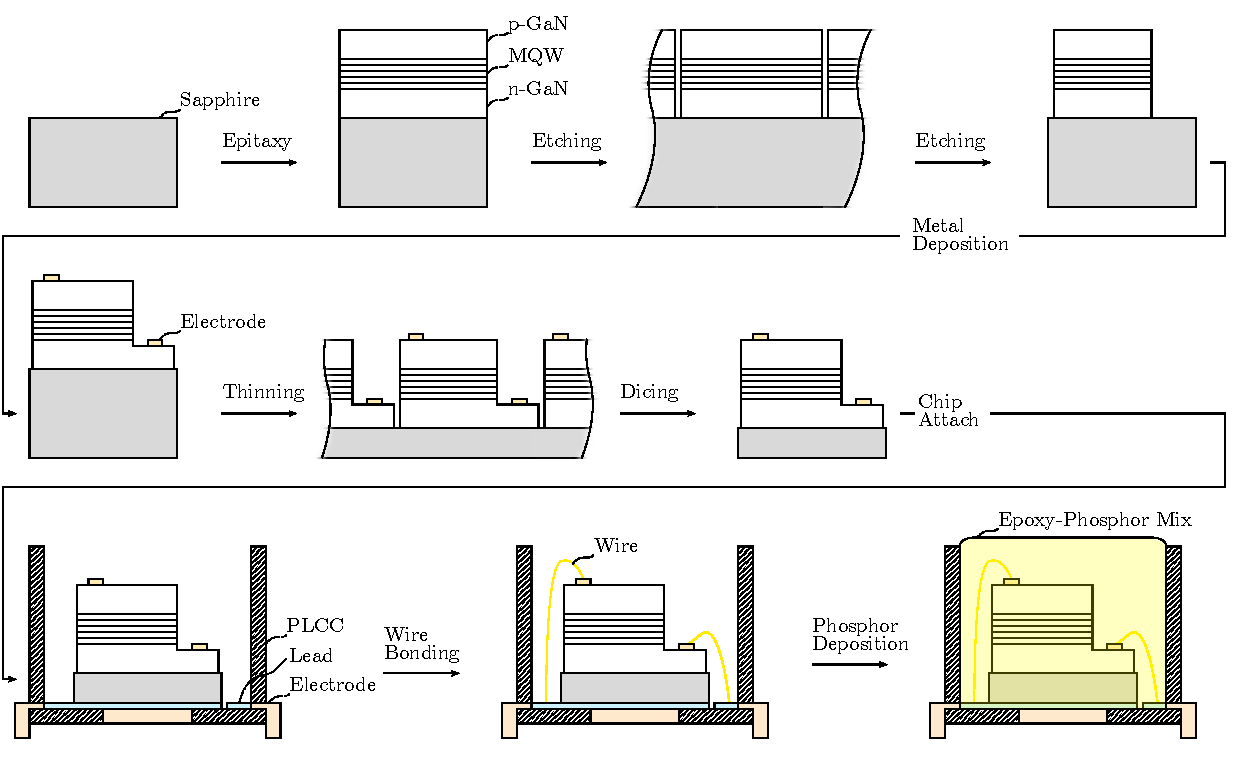
\includegraphics[width=555pt]{./figures/classical_overview_2003.pdf}
            \caption{\textbf{Manufacturing process for a classical LED package with lateral current spreading, circa 2003.} MQW - multiple quantum well; PLLC - plastic leaded chip carrier.}
        \label{fig:manuf_classical_2003}
        \end{figure}
    \end{landscape}
    
    %VERTICAL THIN-FILM FLIP-CHIP

    \begin{landscape}
        \begin{figure}
            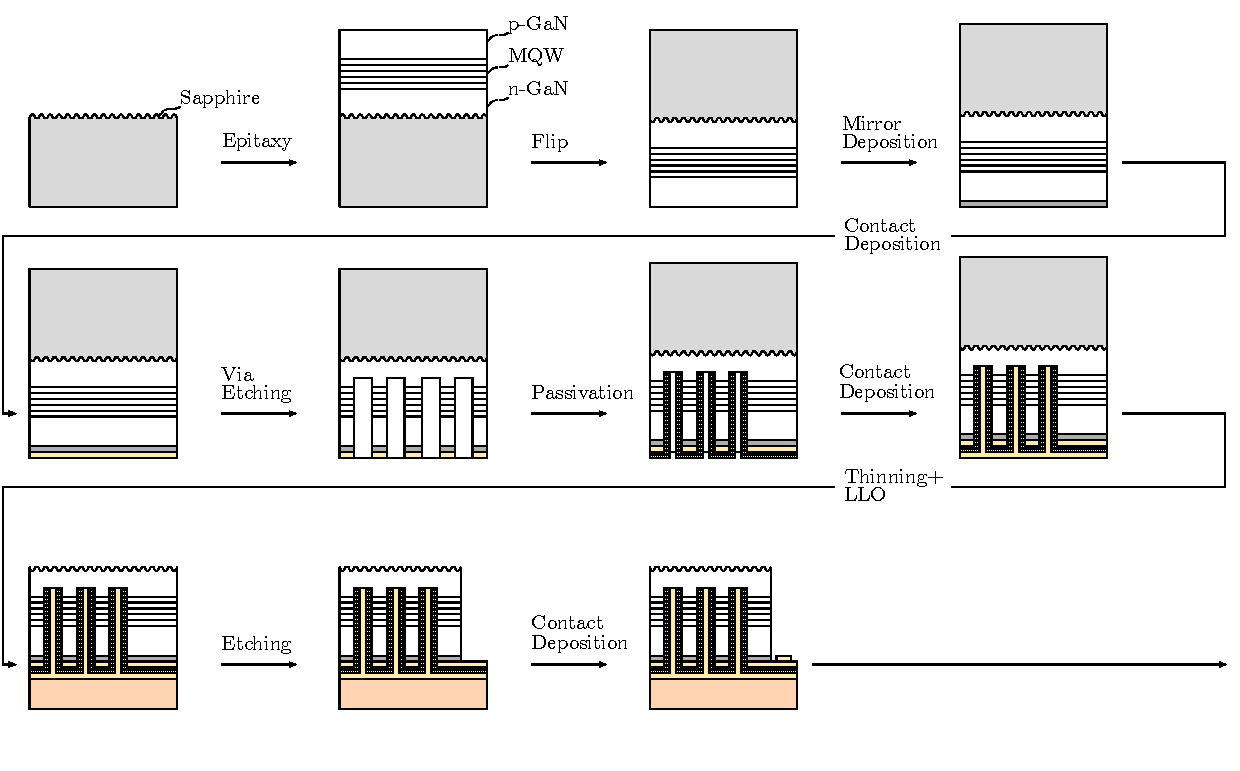
\includegraphics[width=595pt]{./figures/vtf_overview_2012-1.pdf}
            \caption{\textbf{Manufacturing process for a vertical thin-film  package flip-chip LED chip with vertical current spreading, circa 2012. (1/2)} MQW - multiple quantum well; LLO - laser lift-off. Continued in \cref{fig:manuf_vtf_2012-2}}
            \label{fig:manuf_vtf_2012-1}
        \end{figure}
    \end{landscape}

    \begin{landscape}
        \begin{figure}
            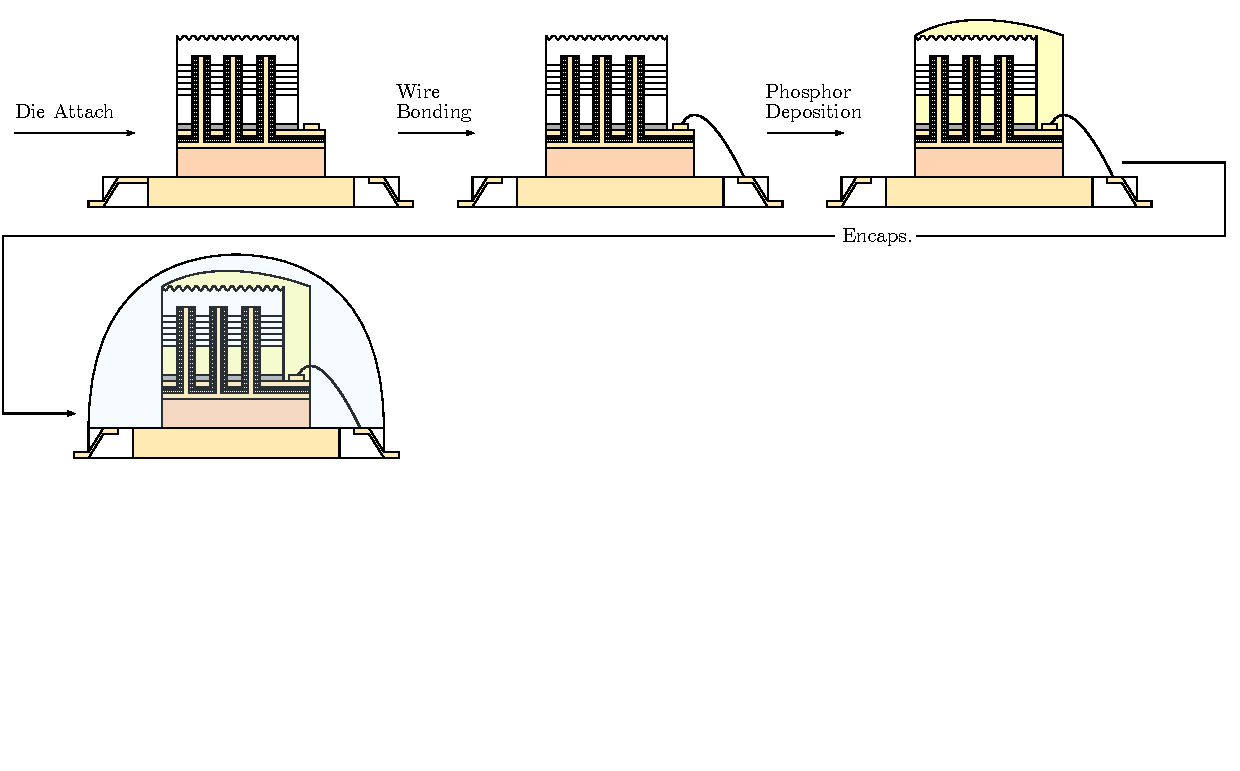
\includegraphics[width=595pt]{./figures/vtf_overview_2012-2.pdf}
            \caption{\textbf{Manufacturing process for a vertical thin-film package flip-chip LED chip with vertical current spreading, circa 2012 (2/2)}. Continued from \cref{fig:manuf_vtf_2012-1}. Encaps. - encapsulation.}
            \label{fig:manuf_vtf_2012-2}
        \end{figure}
    \end{landscape}

    % CHIP-SCALE PACKAGE FLIP-CHIP

    \begin{landscape}
        \begin{figure}
            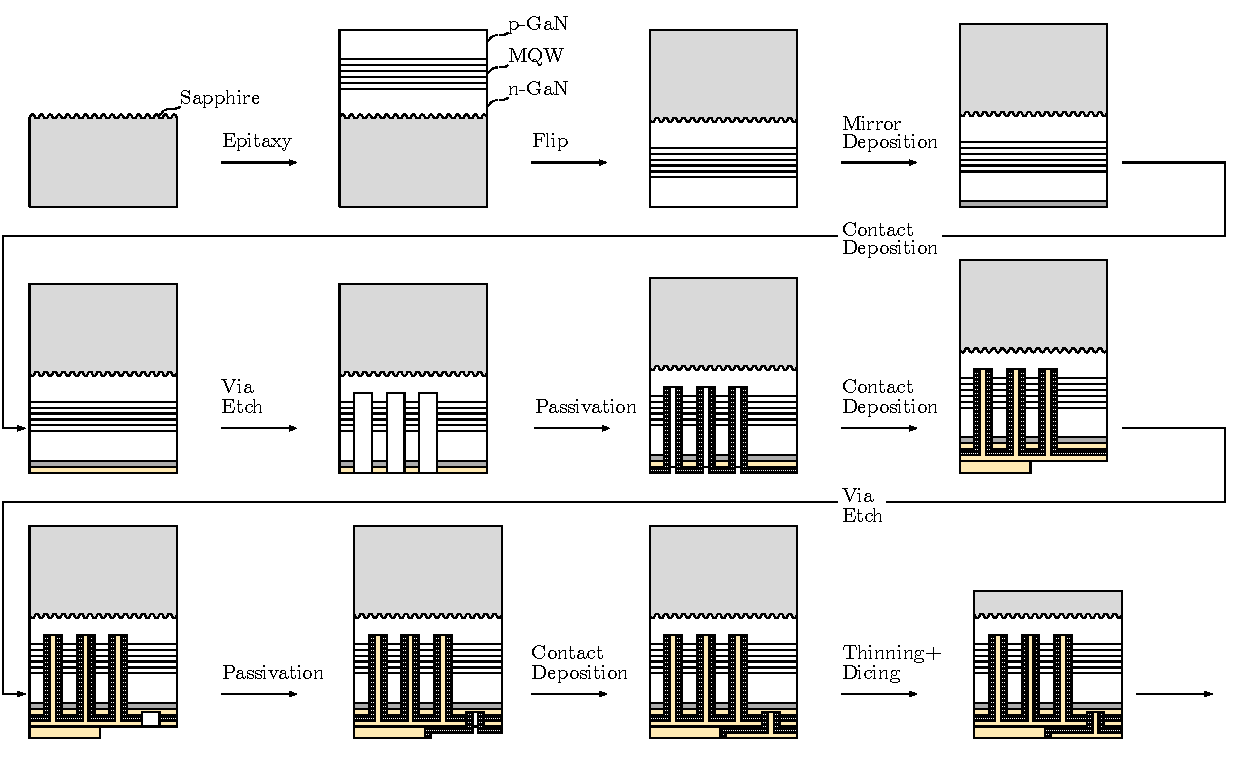
\includegraphics[width=595pt]{./figures/csp_overview_2020-1.pdf}
            \caption{\textbf{Manufacturing process for a chip scale package flip-chip LED chip with vertical current spreading, circa 2020. (1/2)} MQW - multiple quantum well. Continued in \cref{fig:manuf_csp_2020-2}.}
            \label{fig:manuf_csp_2020-1}
        \end{figure}
    \end{landscape}

    \begin{landscape}
        \begin{figure}
            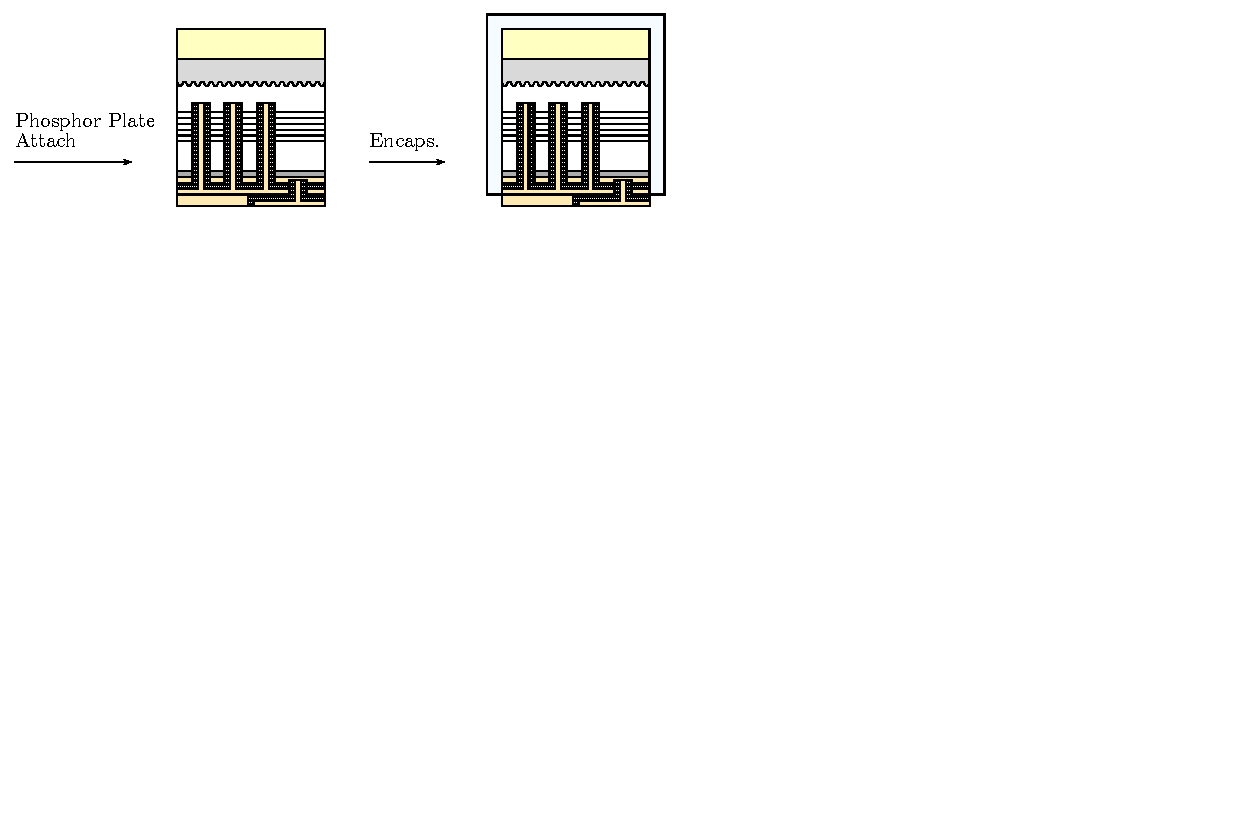
\includegraphics[width=595pt]{./figures/csp_overview_2020-2.pdf}
            \caption{\textbf{Manufacturing process for a chip scale package flip-chip LED chip with vertical current spreading, circa 2020. (2/2)}. Continued from \cref{fig:manuf_csp_2020-1}. Encaps. - encapsulation.}
            \label{fig:manuf_csp_2020-2}
        \end{figure}
    \end{landscape}

\clearpage

\subsection{Historical Progress in Chip Architectures}
\label{sec:chip_architecture}

\begin{figure}[h!]
\centering
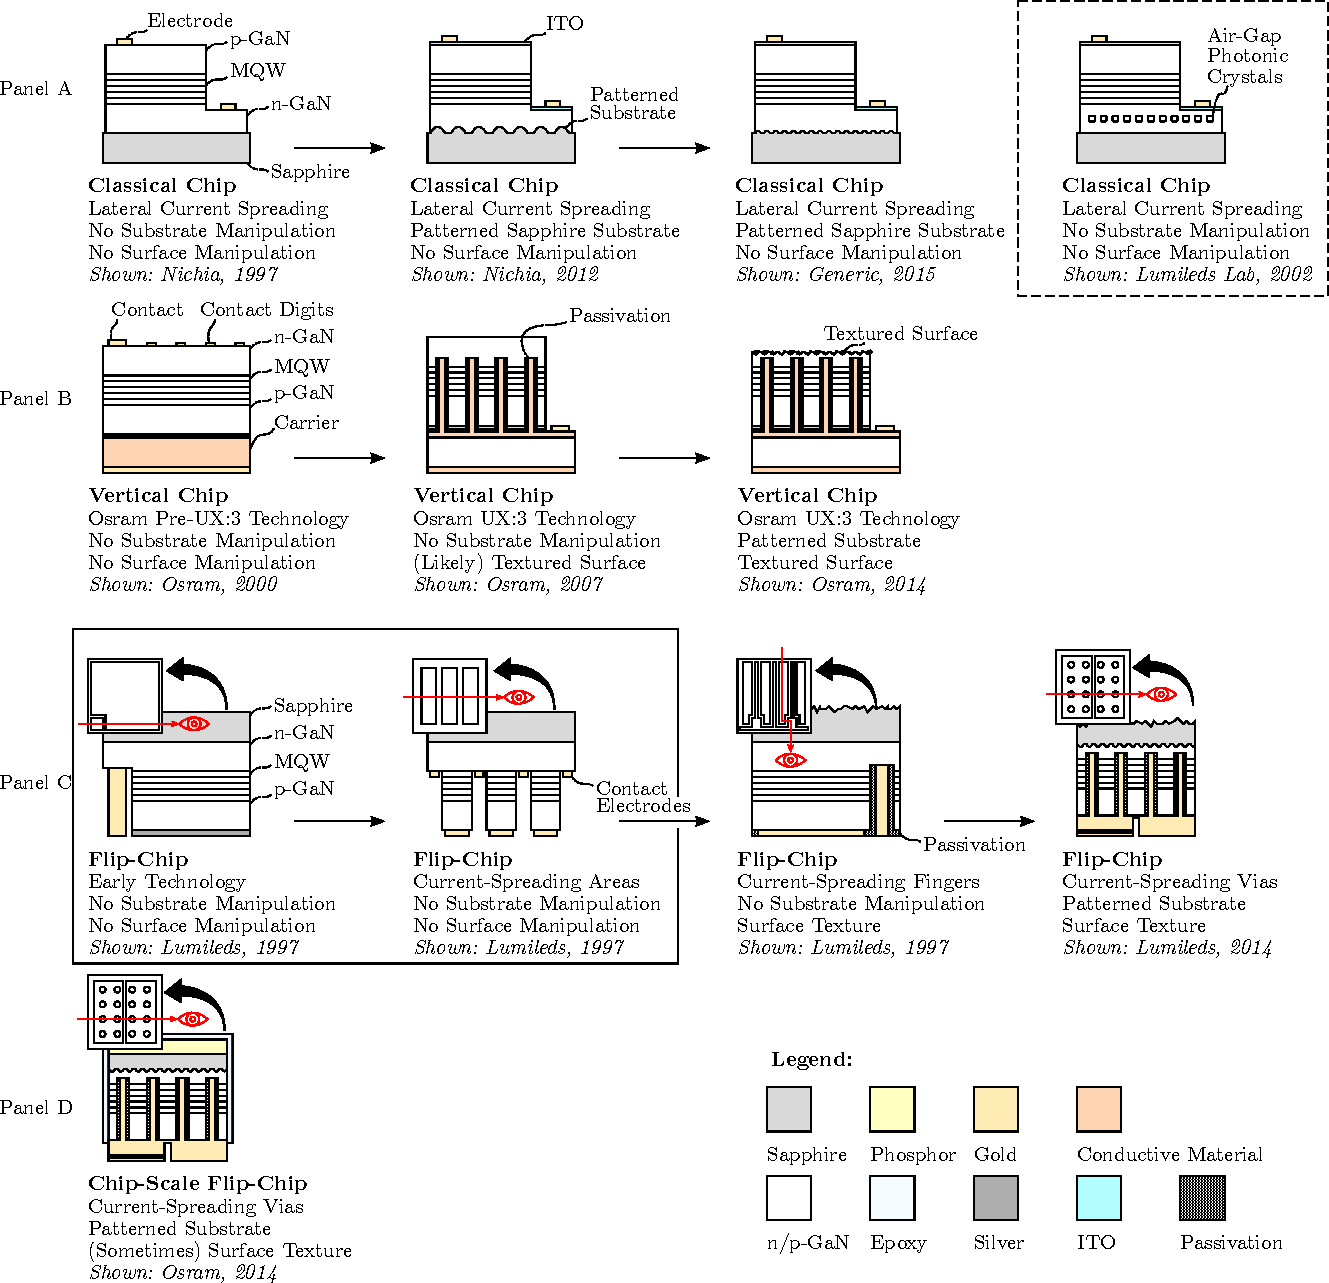
\includegraphics[height=15cm]{figures/chip_architecture_overview.pdf}
\caption{\textbf{Historical evolution of LED chip architectures.} Panel A: classical chip with lateral current spreading; Panel B: Osram’s thin GaN flip-chip (vertical) architecture; Panel C: flip-chip architecture; Panel D: chip-scale package flip-chip architecture. Shown are side views of chips without packages, along a cutaway line best suited to the features of each architecture. The cutaway surface is indicated by a red arrow with an eye on the overlaid top view of each chip. Note that the dimensions are not to scale, and smaller features are greatly exaggerated for clarity. Years indicated correspond to the earliest identified patent priority date. Dashed black frames around certain designs indicate chip designs not brought to large-scale production. Additional context on this figure is provided in \cref{sec:subeff_progress}. Chip architecture abbreviations: TF - Thin-Film; FC - Flip-Chip; CSP - Chip-Scale Package; Material abbreviations: GaN - Gallium Nitride, ITO - Indium Tin Oxide, MQW - Multiple Quantum Well. Source: adapted and compiled from multiple patents and industry publications. See Supplementary Note 16 for the full list of sources and references.}
\label{fgr:chip_architecture_overview}
\end{figure}

\clearpage
\subsection{Historical Progress in Sub-Efficiencies}
\label{sec:subeff_progress}

\begin{figure}[H]
\centering
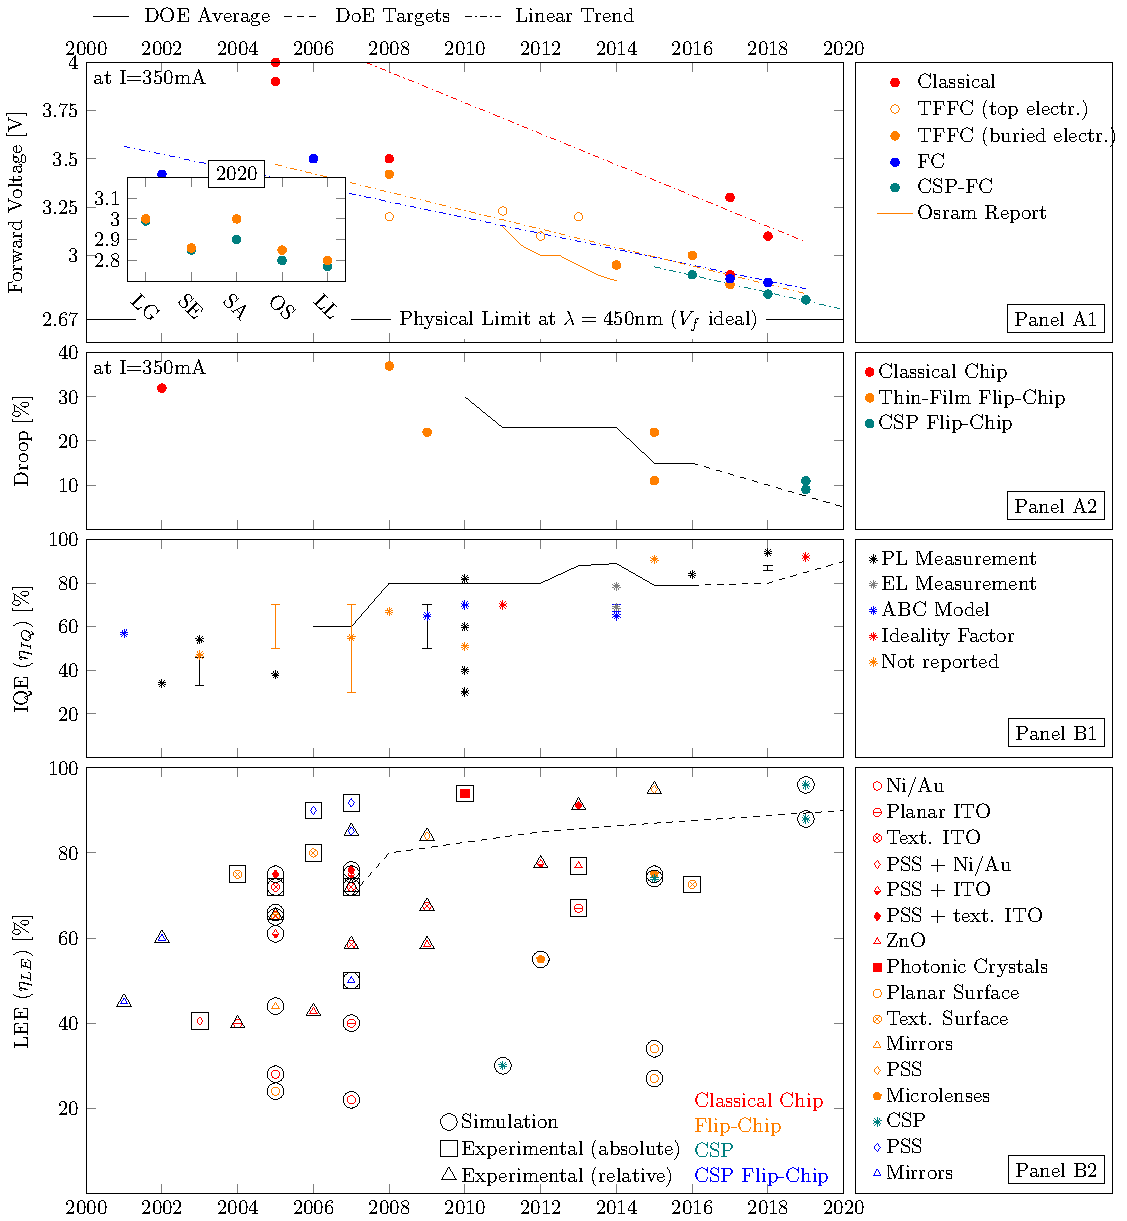
\includegraphics[width=15.5cm]{./figures/subefficiencies_progress.pdf}
\caption{\textbf{Historical improvements in white LED sub-efficiencies.} Panels A1-A2 show data for key metrics used to calculate forward voltage efficiency $\eta_{Vf}$ and droop efficiency $\eta_{droop}$. Panels B1-B2 show data for internal quantum efficiency $\eta_{IQ}$ and light extraction efficiency $\eta_{LE}$. Spectral data related to spectral sub-efficiency is shown in \cref{fig:phosphor_spectrum}. Additional context for the panels is provided below. Source: own synthesis of data from the list of sources provided in \cref{sec:sources}. For an illustration of the different chip architectures shown, compare \cref{sec:chip_architecture}. Data on average device performance adapted from U.S. Department of Energy (DOE) Reports \cite{doe_ssl_multiyear_2007}\cite{doe_ssl_multiyear_2008}\cite{doe_ssl_multiyear_2013}\cite{doe_ssl_rnd_2016}\cite{doe_ssl_rnd_2018} and an Osram company report \cite{beale_leds_2015}.}
\label{fgr:subeff}
\vspace{-20mm}
\end{figure}

\clearpage

\textbf{Panel A1:} This panel shows device forward voltage at a test current of I=350mA, categorized by chip architecture. The physical limit for a blue light wavelength of 450nm without electric pumping is shown for reference. Forward voltage efficiency is computed from this metric as described in \cref{sec:device_performance_metrics}. Data points for devices released in 2020 by various manufacturers are shown in an inset plot for additional context. Note that differences between chip architectures in this plot have become small for all but one company. Chip architecture abbreviations: Acronyms: TFFC - thin-film flip-chip, FC - flip-chip, CSP-FC - chip-scale package flip-chip. Company abbreviations: LG - LG Innotek, SE - Seoul Semiconductor, SA - Samsung, OS - Osram, LL - Lumileds.  \

\textbf{Panel A2:} Efficiency droop at the test current of I=350mA, categorized by chip architecture. Droop efficiency is computed from this metric as described in \cref{sec:device_performance_metrics}. Data has been calculated from luminous intensity curves of respective device datasheets. \

\textbf{Panel B1:} Internal quantum efficiency (IQE) for categorized by type of measurement used. Because it is inherently more difficult to measure IQE than is the case for other sub-efficiencies, this panel shows data categorized by different measurement methods. This is not the case for other panels of this figure. Note that the bump in the DOE Average around 2013 is due to a change in IQE definition laid out in \cite{doe_ssl_multiyear_2013}. Measurement methods abbreviations: PL - Photoluminescence \cite{Shim_2018}, EL - Electroluminescence \cite{Getty_2009}; ABC Model \cite{Karpov_2014}, Ideality Factor \cite{Masui_2010}. “Not reported” denotes data points where the IQE measurement technique was not reported. Whiskers indicate reported ranges, where available. \

\textbf{Panel B2:} Light extraction efficiency (LEE) for different chip architectures by type of specific technology used to improve LEE. The sources for all data points are shown for reference: Simulation - ray-tracing computer simulation; Experimental (absolute) – direct LEE values; Experimental (relative) - relative improvement over baseline chip architecture. Abbreviations: TFFC - Thin-Film Flip-Chip; FC - Flip-Chip; CSP - Chip-Scale Package; ITO - Indium Tin Oxide; ZnO - Zinc Oxide; PSS - Patterned Sapphire Substrate; electr. - electrode; text. - textured.

\textbf{Additional Notes on \cref{fgr:chip_architecture_overview} and \cref{fgr:subeff}}

The data shown in \cref{fgr:subeff} and \cref{fig:phosphor_spectrum} was used to determine the performance of best-in-class devices across different sub-efficiencies. The results of these efficiency calculations are shown in Figures 3-5 in the main text. \cref{fgr:chip_architecture_overview} provides important context by illustrating the associated changes in chip architecture. This show the evolution of LEDs from classical chips with lateral current spreading to chip-scale package flip-chip architectures. We provide two examples:

Panel B2 of \cref{fgr:subeff} shows how light-extraction efficiency can be improved from $\sim40\%$ to $\sim95\%$ by switching from a planar Indium-Tin Oxide (ITO) surface to a patterned sapphire substrate (PSS). This is listed as a spillover in Figure 4 in the main text. Panel A in \cref{fgr:chip_architecture_overview} shows where on the chip these changes take place and provides typical examples of the relevant chip types.

Panel A1 of \cref{fgr:subeff} shows forward voltage was reduced (and therefore forward voltage efficiency increased) over time. This trend is observable both within the same chip architectures and between chip architectures. The most recent data points for 2018-2019 show how classical chips still have the highest forward voltage. Panels A-D in \cref{fgr:chip_architecture_overview} provides typical examples of the relevant chip types.

\clearpage
\subsection{Non-Phosphor-Related LED Innovations}

\cref{tab:innovations_1}-\cref{tab:innovations_2} summarize LED innovations and technology and manufacturing process improvements identified in this study as affecting four white LED sub-efficiencies: forward voltage efficiency, light extraction efficiency, internal quantum efficiency, droop and light conversion efficiency. Note that this table does not include phosphor-related LED innovations affecting spectral efficiency, as these are presented separately in Table 1 in the main text as affecting consumer experience metrics and discussed in detail in \cref{sec:innovation_phosphor}.

\begin{table}[H]
    \caption{\textbf{White LED innovations and technology improvements affecting key device sub-efficiencies.} Note this table is continued in \cref{tab:innovations_2}.}
    \begin{NiceTabularX}{\textwidth}{ |l|X|X|l|l| }
        \hline
        \multicolumn{5}{c}{Forward Voltage Efficiency (FVE) $\eta_{Vf}$} \\
        \hline
            \textit{Year} & \textit{Innovation} & \textit{Area of Improvement} & \textit{Spillover} & \textit{Source} \\
        \hline
            1999 & Indium Tin Oxide \newline Current spreading layer & Contact resistance & Yes & \cite{margalith1999indium}\\
        \hline
            1998 & Digitated electrodes & Contact resistance & No & \cite{steigerwald2001electrode} \\
        \hline
            Ongoing & Epitaxy improvements \newline and better doping & Polarization and \newline bulk resistance & No & I \\
        \hline
            1998 & Silver p-Contacts & Contact resistance & No & \cite{kondoh2001nitride} \\
        \hline
        \multicolumn{5}{c}{Light extraction efficiency (LEE) $\eta_{LE}$} \\
        \hline
            \textit{Year} & \textit{Innovation} & \textit{Area of improvement} & \textit{Spillover} & \textit{Source} \\
        \hline
            $<$ 2003 & Optimization for \newline cavity effects & Reduces self-interference of quantum well & No & I, \cite{Shen2003} \\
        \hline
            1993 & Chip surface randomization & Total reflection and absorption & No & I, \cite{bergh1973surface}\cite{Schnitzer1993} \\
        \hline
            1993 & Thin-film chip architecture & Absorption & No & I, \cite{Schnitzer1993} \\
        \hline
            1996 & Patterned sapphire substrate  & Total reflection and absorption & Yes & I, \cite{Tadatomo2001} \\
        \hline
            Ongoing & Chip design for high LEE & Total reflection and absorption & No & I, \cite{Haerle2004} \\
        \hline
            $\sim$2000 & Silver p-contacts & Absorption & No & I, \cite{kondoh2001nitride} \\
        \hline
        \multicolumn{5}{c}{Internal quantum efficiency (IQE) $\eta_{IQ}$} \\
        \hline
            \textit{Year} & \textit{Innovation} & \textit{Area of improvement} & \textit{Spillover} & \textit{Source} \\
        \hline
            1994 & Double heterostructure & Higher radiative recombination probability & No & \cite{Nakamura1994} \\
        \hline
            1996 & Multiple quantum well & Higher radiative recombination probability & No & \cite{Koike1996} \\
        \hline
            Ongoing & Active region \newline Doping & Radiative recombination probability & No & I, \cite{schubert2018light} \\
        \hline
            Ongoing & Epitaxy \newline Improvements & Radiative recombination probability & No & I \\
        \hline
            Ongoing & Chip architecture \newline Improvements & Radiative recombination probability & No & I \\
        \hline
        \end{NiceTabularX}
        \vspace{2mm}
    \caption*{Note: \textit{Year} column indicates the first instance of application of corresponding invention in white LEDs. 'Ongoing' indicates improvements that are incremental in nature and have been ongoing since the earliest days of LED manufacturing, with no individual breakthroughs identified. \textit{Spillover} column indicates if the innovation involved technology spillovers. \textit{Source} column indicates the source of information about the innovation or improvement, with 'I' indicating expert interviews as such a source.}
    \vspace{-20mm}
    \label{tab:innovations_1}
\end{table}

\begin{table}[H]
    \caption{\textbf{White LED innovations and technology improvements affecting key device sub-efficiencies.} Note that this table continues \cref{tab:innovations_1}.}
    \begin{NiceTabularX}{\textwidth}{ |l|X|X|l|l| }
    \hline
    \multicolumn{5}{c}{Droop $\eta_{droop}$} \\
        \hline
            ongoing & Lower current Density & Current density & No & I \\
        \hline
            ongoing & Epitaxy \newline Improvements & $\ominus/\oplus$ Distribution \newline Defect density & No & I, \cite{bhardwaj2016progress} \\
        \hline
            ongoing & Chip Architecture \newline Improvements  & $\ominus/\oplus$ Distribution \newline Defect density & No & I, \cite{Wildeson2017} \\
        \hline
            $<$ 2017 & Defect getting \newline underlayer & Defect density & No & I, \cite{haller2017burying} \\
        \hline
        \multicolumn{5}{c}{Light conversion efficiency (CE) $\eta_{C}$} \\
        \hline
            \textit{Year} & \textit{Innovation} & \textit{Area of improvement} & \textit{Spillover} & \textit{Source} \\
        \hline
            Ongoing & Lower current density & Current density & No & I \\
        \hline
            Ongoing & Epitaxy \newline Improvements & Charge distribution \newline Defect density & No & I, \cite{bhardwaj2016progress} \\
        \hline
            Ongoing & Chip architecture \newline improvements  & Charge distribution \newline Defect density & No & I, \cite{Wildeson2017} \\
        \hline
            $<$ 2017 & Defect gettering \newline underlayer & Defect density & No & I, \cite{haller2017burying} \\
        \hline
        \end{NiceTabularX}
        \vspace{2mm}
    \caption*{Note: \textit{Year} column indicates the first instance of application of corresponding invention in white LEDs. 'Ongoing' indicates improvements that are incremental in nature and have been ongoing since the earliest days of LED manufacturing, with no individual breakthroughs identified. \textit{Spillover} column indicates if the innovation involved technology spillovers. \textit{Source} column indicates the source of information about the innovation or improvement, with 'I' indicating expert interviews as such a source.}
    \label{tab:innovations_2}
\end{table}

\clearpage
\subsection{Phosphor-Related LED Innovations}
\label{sec:innovation_phosphor}

This section provides additional details for phosphor-related LED innovations identified in this study as affecting both spectral sub-efficiencies and consumer experience metrics. These include a detailed description of the history of those innovations, which we use to identify the details of involved technology spillovers. In addition, spectral data for the first identified white LED products that used those innovations is presented in \cref{fig:phosphor_spectrum}, which we use to calculate consumer experience metrics, as well as LED spectral efficiency.

\textbf{YAG and YGAG Phosphors}

Prior to Nakamura’s invention of highly efficient blue LEDs in the 1990s, Japan’s Nichia Corporation had not sold commercially successful semiconductor products, instead specializing in phosphors for cathode ray tubes (CRT) and fluorescent lamps \cite{nakamura2013blue}  . Nevertheless, extensive firm expertise in this area helped Nichia’s Yoshinori Shimizu formulate the principles of using CRT phosphors to convert blue light from Nakamura’s LEDs into white light in 1994 \cite{shimizu1994sheet}\cite{cho2017white}. By 1996, Shimizu and his colleagues developed \cite{bando1996}\cite{shimizu1999light} the first practical LED application of a well-known Yttrium Aluminium Garnet (YAG) CRT phosphor activated with cerium \cite{blasse1967new}, enabling the first commercial white LED products manufactured and sold by Nichia since late 1996 \cite{bando1998development}\cite{cho2017white}. 

Importantly, the YAG phosphor does not exhibit the spectral properties desirable in general illumination applications (see Figure 6 in the main article). An early solution to this problem, which was first discovered in the late 1967 \cite{holloway1969optical} and suggested for LEDs by the same team at Nichia in 1996 \cite{bando1998development}\cite{shimizu1999light}, was to use the gadolinium-doped red-shifted YAG phosphor (YGAG). Used in combination with red-emitting sulfide phosphors, by 2003 it helped bring to the market the first generation of warm white light LED products, e.g., those produced by Lumileds \cite{Mueller2002}. However, sulfide phosphors led to accelerated deterioration of sensitive parts of LED devices and became less efficient as operating temperatures increased. New chemically stable and non-toxic red phosphors were needed. 

\textbf{258, SLA and SALON phosphors}

In 1997, Hubert Huppertz and Wolfgang Schnick, working at the University of Bayreuth in Germany, synthesized the first compound in a new class of rare earth nitridosilicate materials \cite{Huppertz1997} later dubbed “258” due to a proportion of elements in its chemical formula. The luminescent properties of these materials were identified by the Schnick’s group, by then at Ludwig-Maximilians University of Munich, in 2000 \cite{Hppe2000} after a suggestion made to Schnick at a conference following earlier reports of good luminosity properties of europium-doped compounds \cite{Qiua1998}. U.S.-based LED manufacturer Lumileds applied for a patent for the first class of red LED phosphors based on the 258 nitridosilicate chemistry in 2003 \cite{mueller2004phosphor}. The first use of the 258 phosphor in a commercial “Luxeon” LED package was then reported in a joint publication co-authored by inventors from Lumileds and researchers from the Schnick’s group in 2005 \cite{MuellerMach2005}.

Further efforts in LED phosphor development were directed towards synthesizing a red narrow-band phosphor. Narrow LED emission peak widths yield the highest luminous efficacy of radiation, as in this case less light is emitted in the far-red range of the spectrum in which the human eye is not very sensitive. After synthesizing several narrow-band phosphors emitting in yellow \cite{Hppe2004} and cyan \cite{Kechele2009}, the Schnick’s group identified the local cubic cation coordination structure of the cyan phosphor compound as the reason for its narrow band width \cite{lumi2016narrow}. A search for a structurally analogous nitride compound with the narrow red instead of the cyan emission was undertaken. After several unsuccessful attempts, the sought-after cuboidal nitride compound was found in a 2008 publication led by Francis DiSalvo \cite{Park2008Sr}. Based on information provided in this work, Schnick and colleagues synthesized and studied the spectral properties of a new narrow band red SLA phosphor in 2013 \cite{schmidt2013new}\cite{Pust2014}. The material was introduced in commercial white LED devices by Lumileds in 2015 \cite{lumi2016narrow_whitepaper}. 

The most recent red narrow-band phosphor innovation included in Table 1 and Figure 6 in the main article, indicated as SALON, has been under development during the late 2010s by a group of Austrian and German researchers that included Huppertz, the discoverer of the “258” material, working in collaboration with Osram, another major LED manufacturer \cite{seibald2019phosphor}\cite{Hoerder2019}\cite{Hoerder2020}. The first U.S. patent application for this phosphor was filed in 2017 \cite{seibald2019phosphor}. The SALON phosphor is a derivate of the SLA phosphor. Therefore, it is the only innovation related to consumer experience metrics identified in our study that seemingly not involved technology spillovers.

\textbf{PFS Phosphor}

Down conversion with ultra-narrow-band phosphor can achieve the highest spectral efficiency. However, few such phosphors have been identified, with even less exhibiting desirable material properties such as thermal stability \cite{Phillips2007}. The first commercially successful ultra-narrow-band red phosphor was developed by General Electric (GE). It is based on a potassium fluorosilicate (PFS) compound activated with manganese ions. Its luminescence was first recorded by Adrian Paulusz at GE in 1972 \cite{paulusz1973efficient}. In the early 2000s, while searching for potential new LED phosphor materials for GE’s lighting business at GE Lumination, Emil Radkov rediscovered Paulusz’s findings in the literature. Following extensive research on PFS chemical synthesis and material properties conducted in collaboration with the University of Sofia in Bulgaria, Radkov’s Alma Mater, the PFS phosphor had been under development at GE since 2005 \cite{radkov2006red}\cite{radkov2009red}. This work, supported by public funding from the U.S. Department of Energy (DOE) Solid-State Lighting program \cite{doesslprogram}, resulted in a series of critical improvements in the PFS phosphor properties \cite{Setlur2010}\cite{lyons2012color}, eventually enabling its commercialization under the “TriGain” brand in 2015 \cite{trigain_spectrum}\cite{setlur2015trigain}\cite{Murphy2015}.

\textbf{Quantum Dots for Light Down-Conversion}

Quantum dots (QD) are semiconductor nanocrystals whose quantum size effects make QDs behave as “artificial atoms”. Semiconductor quantum dots were first synthesized in the Soviet Union in 1981 \cite{ekimov1981quantum} and at Bell Labs in the U.S. in 1983 \cite{Rossetti1983}. Luminescent properties of quantum dots were first empirically observed in 1984 \cite{fojtik1984photo} and extensively studied in the early 1990s. The key feature of QD luminescence discovered in those studies is that its colour is determined by the QD particle size, making it possible to create pure monochromatic blue, green and red light sources just by tuning the QD size. The first application of QDs in LEDs was reported in 1994 in an electroluminescent hybrid QD-polymer LED. However, this LED type could not be used in general illumination due to its very low luminous efficacy. An alternative application of QDs as a kind of a “phosphor” for light down conversion from an LED light source was proposed in the early 2000s as part of the U.S. Department of Energy (DOE)-funded “A Revolution in Lighting“ project at Sandia National Laboratory \cite{simmonsfinal}. This concept was successfully demonstrated by Sandia researchers on a commercial LED in 2003 \cite{shea_rohwer_development_2004}\cite{noauthor_sandia_nodate} and was swiftly taken up and advanced further by a group in Taiwan \cite{Chen_2005}\cite{Hsueh_Shih_Chen_2006} The first commercial application of QDs in an LED lamp was brought about by a collaboration between an MIT-born startup QD Vision and the U.S.-based luminaire manufacturer Nexxus Lighting in 2009 \cite{ledprof_nexxusqd}, \cite{bourzac2013quantum}. However, rapid advances in the spectral and conversion performance of down-conversion phosphors and high manufacturing cost of quantum dots resulted in the discontinuation of this product. After finding market success in display backlighting first demonstrated by Samsung in 2010 \cite{Jang2010} and commercialized by QD Vision in Sony television sets in 2013 \cite{bourzac2013quantum}, QDs returned to the general lighting market in products offered by Lumileds \cite{noauthor_global_2017}\cite{noauthor_quantum_2020} around 2017 and Osram in 2019 \cite{osramqdots} in the form of mid-power LED packages that combined QDs with traditional phosphors for light down conversion.

\subsection{Spectral Data for Phosphors}

\begin{figure}[H]
	\centering
    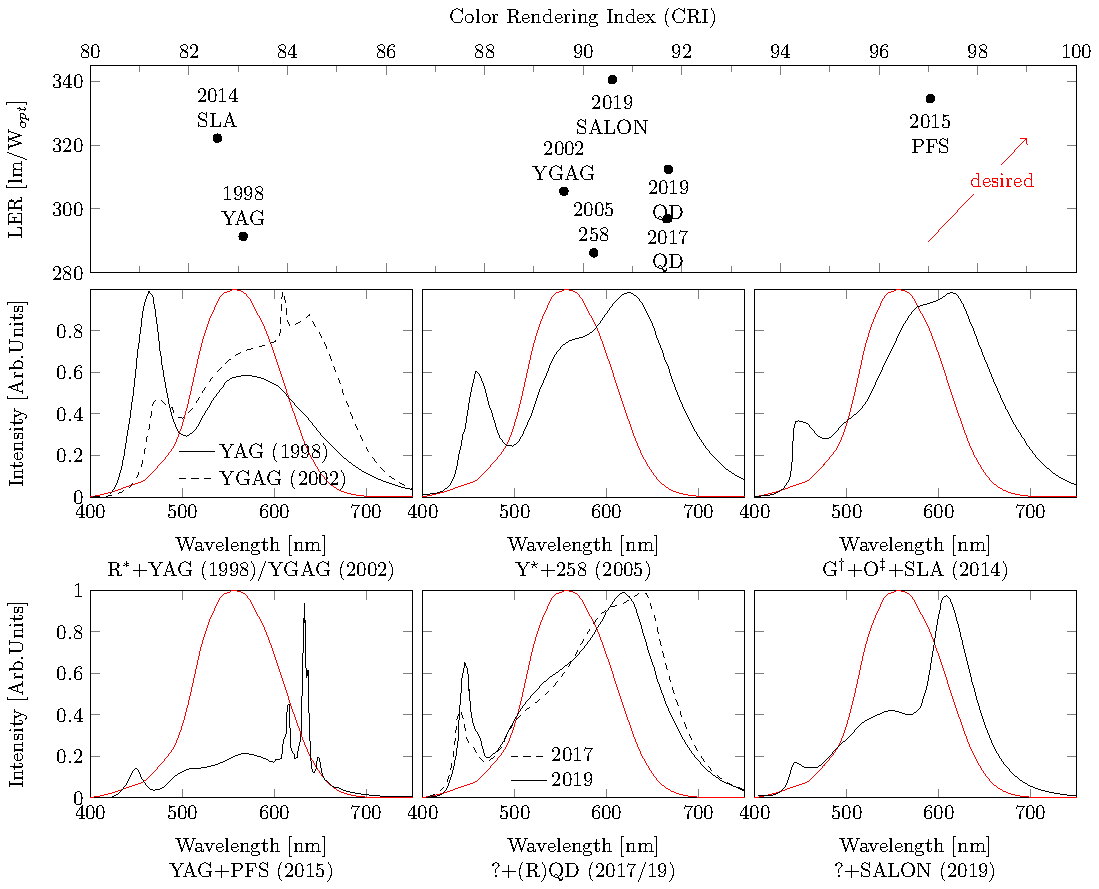
\includegraphics[width=0.9\textwidth]{./figures/phosphor_spectrum-comparison.pdf}
	\caption{\textbf{Spectral data and additional consumer experience metrics for the earliest identified representative white LED products with published spectral data.} Corresponding LED products that used phosphor innovations listed in Table 1 in the main article are each indicated by the phosphor label and spectral data publication year. Top panel: Luminous efficacy of radiation (LER) and colour rendering index (CRI) of white LED devices represented in Figure 6 in the main article. The desirable direction of improvements towards higher LER at higher CRI is indicated by a red arrow. Metrics were calculated from spectral data shown in the bottom panels using the \texttt{colour-science} package for Python \cite{colour-science_software}. Bottom two rows of panels: spectral data for the first identified LED products that used phosphor innovations listed in Table 1 in the main article. The luminosity function \cite{cie-term-lumeff}, describing the wavelength-dependent sensitivity of the human eye, is shown for reference in red in each panel. Peaks or large tails of the device emission spectrum at the far ends of the luminosity function are not desirable, as the photons of the corresponding energy are lost to the human eye and count towards the spectral loss channel. Plot legends indicate the years of publication of the spectral data and phosphor mixtures used in corresponding LED devices, with the following designations for additional phosphor mix components: ? -  other parts of phosphor mixture not disclosed, G$^*$ - \ch{CaSrS:Eu^{2+}}, Y$^\star$ - $\beta-$SiAlON:Eu$^{2+}$, G$^\dagger$ - \ch{Lu_3Al_5O_{12}:Ce^{3+}}, O$^\ddagger$ - \ch{(Ba,Sr)_2Si_5N_8:Eu^{2+}}. Source (top panel): own elaboration based on spectral data. Arb. Units - Arbitrary Units, defined as the ratio of radiation intensity at a wavelength compared to the highest point in the spectrum. Sources: top panel - own elaboration based on spectral data; bottom two panels: adapted from published spectral data for LEDs with the following phosphors: YAG \cite{bando1998development}, YGAG \cite{Mueller2002}, 258 \cite{MuellerMach2005}, SLA \cite{Pust2014}, PFS \cite{trigain_spectrum}, QD \cite{lumileds2016qd}\cite{osram2019qd}, SALON \cite{Hoerder2019}.}
\label{fig:phosphor_spectrum}
\end{figure}

\clearpage
\subsection{Full List of Sources for Figures}
\label{sec:sources}

\begin{table}[h!]
\captionsetup{justification=raggedright,singlelinecheck=false}
    \caption{List of sources for Figure 1.}
    \begin{NiceTabularX}{\textwidth}{|l|X|}
    \hline
    \textit{Technology} & \textit{References} \\
    \hline
    LED & Own research, compare \cite{zenodo_weinold_led_history} \\
    \hline
    CFL (<1984) & \cite{Bouwknegt1982}\cite{Vrenken1983} \\
    \hline
    CFL (1984-2011) & \cite{eger2018origin} \\
    \hline
    CFL (>2011) & \cite{Guan2015} \\
    \hline
    Fire, Incandescent, HID & \cite{azevedo2009transition} augmented by own calculations based on \cite{benesch1905beleuchtungswesen} \\
    \hline
    Max. efficacy & \cite{Murphy2012} \\
    \hline
    \end{NiceTabularX}
    \vspace{2mm}
    \caption*{Abbreviations: CFL - Compact Fluorescent Lamp, HID - High-Intensity Discharge}
\end{table}

\begin{table}[h!]
\captionsetup{justification=raggedright,singlelinecheck=false}
    \caption{List of sources for Figure 2.}
    \begin{NiceTabularX}{\textwidth}{|l|X|}
    \hline
    \textit{Source} & \textit{References} \\
    \hline
    Stiftung Warentest (Germany) & \cite{Warentest2008}\cite{Warentest2009_1}\cite{Warentest2009_2}\cite{Warentest2010_1}\cite{Warentest2010_2}\cite{Warentest2011}\cite{Warentest2012}\cite{Warentest2013}\cite{Warentest2014_1}\cite{Warentest2014_2}\cite{Warentest2015}\cite{Warentest2016_1}\cite{Warentest2016_2}\cite{Warentest2018} \\
    \hline
    Konsument (Austria) & \cite{Konsument2010} \\
    \hline
    Which (UK) & \cite{Which2020} \\
    \hline
    Industry Periodical & \cite{PM2020} \\
    \hline
    Government Report (US) & \cite{national2013assessment} \\
    \hline
    \end{NiceTabularX}
\end{table}

\begin{table}[h!]
\captionsetup{justification=raggedright,singlelinecheck=false}
\caption{List of sources for Figure 3.}
    \begin{NiceTabularX}{\textwidth}{|l|X|}
    \hline
    \textit{Publication Type} & \textit{References} \\
    \hline
    Scientific Publications & \cite{plossl2010wafer}\cite{bierhuizen2007performance}\cite{gencc2019distributed}\cite{chong2014performance} \\
    \hline
    Patents & \cite{patent1999uemura}\cite{patent1998takaoka}\cite{patent1999komaki}\cite{patent1999komaki}\cite{ludowise2006resonant}\cite{camras2005iii}\cite{steigerwald2004contacting} \\
    \hline
    Other Publications & \cite{craford2015}\cite{sun2016}\cite{yole2013packaging} \\
    \hline
    \end{NiceTabularX}
\end{table}

\clearpage

\begin{table}[h!]
\captionsetup{justification=raggedright,singlelinecheck=false}
\caption{List of sources for Figure 6.}
    \begin{NiceTabularX}{\textwidth}{|l|l|l|X|}
    \hline
    \textit{Phosphor/QD} & \textit{Company} & \textit{YOI} & \textit{Reference} \\
    \hline
    YAG & Nichia & 1998 & \cite{bando1998development} \\
    \hline
    YGAG & Lumileds & 2002 &  \cite{Mueller2002} \\
    \hline
    258 & Lumileds & 2005 & \cite{MuellerMach2005} \\
    \hline
    SLA & Lumileds & 2014 & \cite{Pust2014} \\
    \hline
    PFS & GE & 2015 & \cite{Murphy2015} \\
    \hline
    QD & Lumileds & 2017 & \cite{lumileds2016qd} \\
    \hline
    Salon & Osram & 2019 & \cite{osram2019qd} \\
    \hline
    SALON & Osram & 2019 & \cite{Hoerder2019} \\
    \hline
    \end{NiceTabularX}
\end{table}

\begin{table}[h!]
\captionsetup{justification=raggedright,singlelinecheck=false}
    \caption{List of sources for \cref{fgr:subeff}.}
    \begin{NiceTabularX}{\textwidth}{|l|X|}
    \hline
    \textit{Panel (Sub-Eff.)} & \textit{References} \\
    \hline
    Panel A1 (FVE) & \cite{nichia2001data}\cite{lumi2003lumi}\cite{gen2005data}\cite{candlepwr2005data}\cite{lumi2006data}\cite{lumi2007data}\cite{nichia2008data}\cite{lumi2008data}\cite{osram2008data}\cite{jeong2011high}\cite{osram2012data}\cite{osram2013data}\cite{osram2014data} \newline \cite{lumi2016data_1}\cite{lumi2016data_2}\cite{epistar2017data}\cite{osram2017data_1}\cite{osram2017data_2}\cite{samsung2017data}\cite{samsung2018data}\cite{osram2018data}\cite{epistar2018data}\cite{lumi2019data} \\
    \hline
    Panel A2 (Droop) & Data calculated from luminous intensity curves of respective device datasheets: \cite{datasheet_osram_topled}\cite{osram2008data}\cite{osram2008gdplus}\cite{osram2018csp}\cite{datasheet_lumileds_lux1}\cite{lumi2008data}\cite{lumi2016data_1}\cite{lumi2016data_2}\cite{samsung2018data} \\
    \hline
    Panel B1 (IQE) & Data extracted from respective device datasheets and scientific publications (for a complete list, compare \cite{zenodo_weinold_led_history}). Additional data was extracted from government reports: \newline
\cite{doe_ssl_multiyear_2006}\cite{doe_ssl_multiyear_2007}\cite{doe_ssl_multiyear_2008}\cite{doe_ssl_multiyear_2009}\cite{doe_ssl_multiyear_2010}\cite{doe_ssl_multiyear_2011}\cite{doe_ssl_multiyear_2012}\cite{doe_ssl_multiyear_2013}\cite{doe_ssl_multiyear_2014}\cite{doe_ssl_rnd_2015}\cite{doe_ssl_rnd_2016} \\
    \hline
    Panel B2 (LEE) & \cite{lee2005analysis}\cite{krames2007status}\cite{Jang2004}\cite{Horng2013}\cite{Liao2010}\cite{HungWenHuang2005}\cite{Leem2007}\cite{Huang2008}\cite{Wang2009}\cite{Huh2003}\cite{Horng2008}\cite{Gao2008}\cite{Chang2003}\cite{Zhou2012} \newline \cite{ChunJuTun2006}\cite{Hua2009}\cite{Matioli2010}
\cite{lee2005analysis}\cite{Zhu2015}\cite{Ding2015}\cite{Taki2019}\cite{Shchekin2006}\cite{Hu2016}\cite{Horng2010}\cite{Lin2016}\cite{Yue2018}\cite{Zhao2012}\cite{Zhu2015}\newline \cite{Ding2015}\cite{wierer2001high}\cite{Steigerwald2002}\cite{DaeSeobHan2006}\cite{Wang2006}\cite{Lee2007}\cite{Shen2007}\cite{Huang2006}\cite{Zhmakin2011} \\
    \hline
    \end{NiceTabularX}
\end{table}

\begin{table}[h!]
\captionsetup{justification=raggedright,singlelinecheck=false}
    \caption{List of sources for \cref{fig:haitz_new}.}
    \begin{NiceTabularX}{\textwidth}{|l|X|}
    \hline
    \textit{Metric} & \textit{References} \\
    \hline
    Cost & \cite{doe2010solid}\cite{doe2011solid}\cite{doe2012solid}\cite{doe2013solid}\cite{doe2014solid}\cite{doe2015solid}\cite{doe2016solid} \\
    \hline
    Flux & \cite{haitz2007seoul}\cite{haitz2010osram}\cite{haitz2010lumi-1}\cite{haitz2010cree}\cite{haitz2011lumi-1}\cite{haitz2014nichia}\cite{haitz2015cree-1}\cite{haitz2015cree-2}\cite{haitz2018cree}\cite{haitz2019osram}\cite{haitz2019lumi-1}\cite{haitz2019lumi-1}\cite{haitz2020lumi-1}\cite{haitz2013cob}\cite{haitz2016cob}\cite{haitz2017cob}\cite{haitz2019cob}\cite{haitz2019lumi-1}\cite{haitz2019lumi-2} \\
    \hline
    \end{NiceTabularX}
\end{table}



\clearpage
\section{Supplementary Methods}

\subsection{Literature Review Process}
\label{sec:litrev}

At the first stage of the comprehensive literature review described in section 7.2 in the main text, we conducted a search in specialized patent and publication databases for the most highly cited and/or relevant publications and patents containing information about innovations and overall historical progress in white LED lighting technology.

As several key reviews of technological progress in this field show, the dominant design of white LED lighting that emerged as a result of this progress and diffused at global scale in the lighting market is the GaN-based warm white phosphor-converted LED. See also \cref{sec:prev_lit} for a review of these publications. We therefore decided to focus our analysis exclusively on the evolution of this variation of white LED lighting technology as the only variation that has achieved global market success. Accordingly, we restricted our literature search only to publications focused on GaN-based LED lighting by excluding LEDs with other prominent semiconductor material compositions (i.e., GaAsP, AlGaInP, GaAlAs, ZnO, and perovskites), and on applications of LEDs in lighting by excluding other applications related to solar energy, lasers, or emittance in non-visible parts of the spectrum (e.g., ultraviolet LEDs).

The search was conducted through the \textit{Elsevier Scopus} database using the query provided in \cref{tab:scopus}. The exclusion filters placed additional restrictions on topical areas to focus the search outcomes only on the scientific and engineering basis of LED technology. The top 300 most highly cited papers were analyzed in the outcomes of this search both for their own content, and as an input to the second stage of the literature search described in section 7.2 of the main text that ensured the comprehensiveness of our findings: an iterative ‘snowballing’ search for backward citations in the publications identified at the first stage.

\begin{table}[h!]
\caption{Elsevier Scopus advanced search query.}
\begin{pseudocode}
TITLE-ABS-KEY(("light-emitting" OR "light emitting") W/2 diode*)
AND NOT
TITLE-ABS-KEY(solar OR violet OR laser)
AND NOT
TITLE-ABS-KEY(perovskite OR GaAsP OR AlGaInP OR GaAlAs OR ZnO)
AND NOT
TITLE-ABS-KEY(organic OR OLED* OR polymer*)
AND NOT
SUBJAREA(ARTS OR BUSI OR DECI OR ECON OR PSYC OR SOCI)
AND NOT
SUBJAREA(MEDI OR NURS OR VETE OR DENT OR HEAL OR MULT)
AND NOT
SUBJAREA(AGRI OR BIOC OR IMMU OR NEUR OR PHAR)
AND NOT
SUBJAREA(envi OR EART OR comp)
\end{pseudocode}
\label{tab:scopus}
\vspace{-4mm}
\end{table}

Additional search was conducted in patent databases \textit{The Lens} and \textit{Google Patents}. The search was restricted to a relatively broad CPC patent class H01L 33 (‘Semiconductor devices with at least one potential-jump barrier or surface barrier specially adapted for light emission […]’) and its constituent subclasses, focusing on most highly cited granted patents in this patent class and manually excluding those of them that were not relevant to white LEDs. In practice, this meant that the first-stage patent search was restricted to patents granted after 1990. 

Finally, to complement the search in publications and patents, we also surveyed the archived websites of key LED manufacturers for any materials dedicated to their interpretation of LED history, history of their own products, and major product announcements.

\clearpage

\subsection{Metrics for Quantifying Technological Progress in LEDs}
\label{sec:metrics}

\textbf{Motivation for Metrics Selection}

Investigating the sources of rapid progress in LED technology over the past decades, in which white LEDs have come to dominate the lighting market \cite{zissis2021}, requires selecting appropriate metrics for tracking and quantifying this progress. The choice of metrics affects both what data sources can be used in the analysis and which research methodologies can be used to calculate and analyse such metrics. We select the metrics based on the following two general criteria. First, we focus only on metrics widely accepted and reported in industry. This is because metrics proposed in the scientific literature, but not reported by device manufacturers, cannot be used to compare the performance of commercial LED devices over time. Second, the chosen metrics must be useful for understanding the impact of individual technological improvements on relevant performance and cost characteristics.

Historically, the progress in LED technology has been commonly described by pointing to impressive improvements in LED device performance, more specifically device brightness, as well as electrical efficiency, and manufacturing cost reductions \cite{Taki2019}. However, metrics related to the quality of light, such as the perceived temperature of a white light source and its ability to faithfully render colours, have also played a significant part in the market adoption of new lighting technologies \cite{Menanteau2000,Sandahl2006,CAIRD2008,murphy2012governing} and received substantial attention in LED research and development efforts \cite{azevedo2009transition,cho2017white}. Therefore, a comprehensive analysis of the evolution in white LED technology must take into consideration advances in 1) physical device performance; 2) consumer experience; and 3) LED device manufacturing costs. Next, we introduce and discuss the metrics that we use to track progress in each of these three areas.

\textbf{Distinction between Metrics of Efficiency and Consumer Experience}

We use a well-established distinction between the two types of LED lighting technology performance metrics. Those metrics which are related to the spectrum of the light source only ("color quality metrics" \cite{DLC_SSL_Requirements}\cite{dilaura2011lighting}), we group under the term consumer experience metrics. Those metrics, which are determined by the number and energy of photons leaving the device (as a function of the number of electrons entering it), we group under the term LED efficiency metrics. As such, our distinction is physical at the fundamental level. This follows existing literature on the technological progress in solid-state lighting \cite{tsao2010solid}. We describe these metrics in detail in \cref{sec:device_performance_metrics}-\cref{sec:metrics_consumer}.

\textbf{"Haitz's Law"}

A highly cited and frequently called-upon metric is \textit{flux per package}, as described in what has become known as Haitz's law. An observation rather than a law of nature, it describes increasing device performance and decreasing manufacturing cost. Originally introduced in 2000 \cite{haitz1999case}, it has been updated frequently since then. Unfortunately, the way Haitz's law is frequently used is  problematic due to the misleading conclusions it suggests. While the original version presented by Haitz displays the increasing performance of light-emitting diode chips, the graphs have been extended with datapoints from lamps which contain an unspecified number of chips. The metric therefore loses its value in describing technological progress at the chip-level. The continuing rise in performance inferred from this chart is disconnected from the actual, much lower, performance of single chips \cite{weinold2021compound}. This is shown in \cref{fig:haitz-org}-\cref{fig:haitz_new}.

\begin{figure}[h!]
\vspace{-10mm}
    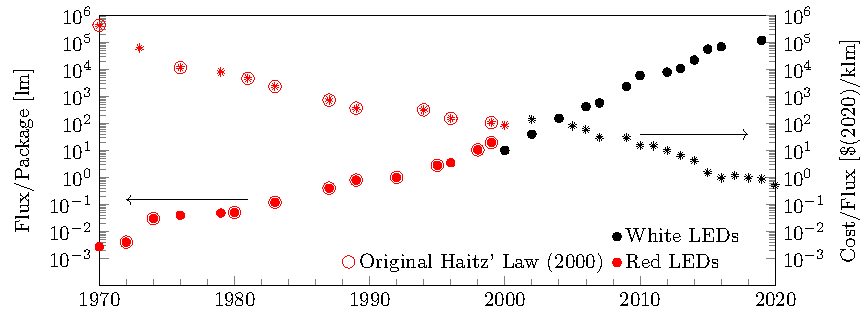
\includegraphics[width=0.9\textwidth]{./figures/haitz_law_old_both.pdf}
    \caption{\textit{"Haitz's Law"}, as it is often reproduced in literature. The original data by Haitz for red LEDs from 2000 is indicated for reference. Note the different range on the horixontal axis compared to \cref{fig:haitz_new}. Sources: \cite{haitz1999case}\cite{haitz2011solid} and  \cref{fig:haitz_new}.}
    \label{fig:haitz-org}
\end{figure}

\begin{figure}[h!]
    \centering
    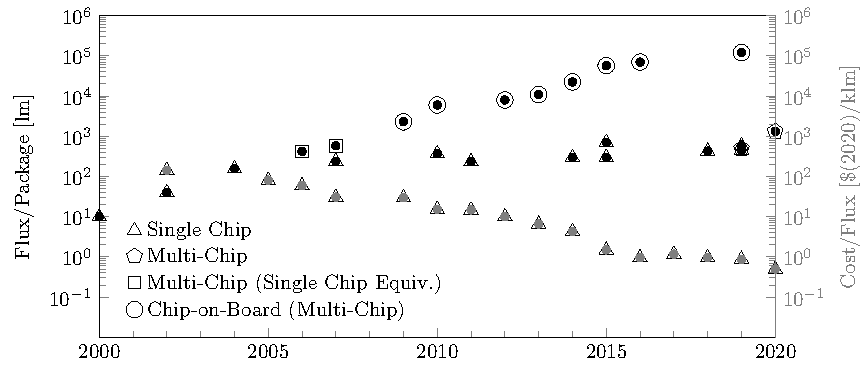
\includegraphics[width=0.85\textwidth]{./figures/haitz_law_white.pdf}
    \caption{Corrected version of \textit{"Haitz's Law"}. Note that the increase in flux per single chip is not increasing as starkly as the flux for multi-chip packages. Shown are datapoints for best commercial performers. See \cref{sec:sources} for the full list of sources and references.}
    \label{fig:haitz_new}
\end{figure}


\clearpage
\subsection{Device Performance Metrics}
\label{sec:device_performance_metrics}

During the years following the market introduction of white LEDs, the primary metric of progress in solid-state lighting was typically luminous flux. This was because the luminous flux (total brightness) of early white LEDs was too small to allow for the economical combination of multiple LEDs into lamps for general illumination purposes. In 2000, the highest performing devices yielded around 10 lm, just below the output of a candle as defined in the unit candela (1 cd=12.57 lm) \cite{haitz2011solid}. Progress in this metric was commonly rendered together with the associated reduction in retail prices as “Haitz’s Law”\cite{haitz1999case,haitz2011solid}, which we discuss in \cref{sec:metrics}. Today, however, the devices with the highest performance yield in excess of 1600 lm, the equivalent of a 100 W incandescent bulb \cite{cree2020bright}. LED brightness has thereby become sufficient to enable the construction of lamps from multiple LED devices, with contemporary improvements focusing instead on higher efficiency and quality of light instead of brightness. Even though a large number of scientific publications and industry periodicals continue to focus on brightness as a metric of progress in lighting, we find that, at this point in time, this metric is insufficient to capture the complexity of the multitude of efficiency improvements that have been driving the overall LED efficiency \cite{weinold2021compound}. Specifically, the stagnating levels of luminous flux in the highest performing devices do not capture the outcomes of a major area of LED research, which is improving electrical efficiency at constant brightness.

We therefore use a combination of the total device efficiency ("lamp efficiency") and the sub-efficiencies that describe different physical loss channels within the device to describe progress in LED technology. In line with previous publications \cite{schubert2018light,tsao2010solid}, we use the following sub-efficiencies: forward voltage efficiency $\eta_{V_f}$, light extraction efficiency $\eta_{LE}$, internal quantum efficiency $\eta_{IQ}$, droop $\eta_{droop}$, conversion efficiency $\eta_{C}$, spectral efficiency $\eta_{S}$. The equations defining these sub-efficiencies are provided below. The overall efficiency ("Lamp Efficiency") $\eta_L$ of a light-emitting diode package is the product of all considered sub-efficiencies:
%
\begin{equation}
    \eta_L = \prod_{i=(V_f, \dots, S)} \eta_i
\end{equation}
%
This metric describes the cumulative electrical and optical losses within the device, as well as the light conversion losses in the phosphor layer.

\textbf{Forward Voltage Efficiency $\eta_{V_f}$}

Device forward voltage efficiency\footnote{"Joule Efficiency" $\epsilon_J$ in Tsao et al. \cite{tsao2010solid}} (FVE) describes all electrical losses at the interface between the electrodes and the semiconductor and in the bulk. These losses can be due to tunneling and Ohmic resistance at the interface, as well as Ohmic resistance and other electrical losses within the bulk of the semiconductor. It is defined as
%
\begin{equation}
    \eta_{V_f} = \frac{E_{h\nu}}{V_f}
\end{equation}
%
where $E_{h\nu}$ denotes the photon energy and $V_f$ is the diode forward voltage \cite{schubert2018light}\cite{tsao2010solid}.

\textbf{Light Extraction Efficiency $\eta_{LE}$}

LED light extraction efficiency (LEE) describes the  losses due to absorption in the material after electron-hole recombination and the associated emission of a photon. It is defined as
%
\begin{equation}
    \eta_{LE} = \frac{P_{opt}}{P_{int}} = \frac{\text{\# of photons out/s}}{\text{\# of photons created/s}}
\end{equation}
%
where $P_{opt}$ is the optical power emitted from the device and  $P_{int}$ is the optical power emitted from the active region into other parts of the device (internal) \cite{schubert2018light}\cite{tsao2010solid}.

\textbf{Internal Quantum Efficiency $\eta_{IQ}$}

Internal quantum efficiency (IQE) describes non-radiative recombinatory processes in the semiconductor bulk. It is defined as
%
\begin{equation}
    \eta_{IQ} = \frac{\# \text{of photons created/s}}{\# \text{of electron-hole pairs injected/s}}
\end{equation}

\textbf{Droop $\eta_{droop}$}

Efficiency droop describes the decrease of LED internal quantum efficiency at high current densities, which is caused by a number of different physical effects\cite{David2020}. This energy loss channel is often treated separately from internal quantum efficiency in the literature due to its importance in high-power devices. It is defined as
%
\begin{equation}
    \eta_{droop} = 1 - \frac{\eta_{IQ}}{\eta_{IQ}(A \rightarrow 0)}
\end{equation}
%
where $\eta_{IQ}(A \rightarrow 0)$ denotes the internal quantum efficiency at low current densities. In practice, droop is often given as the percentage difference between the ideal luminous intensity curve $\phi_{ideal}$ and the real luminous intensity curve $\phi$ at a set diode test current $A_{test}$
%
\begin{equation}
\label{eqn:droop}
    D = \frac{\phi_{ideal}(A_{test})-\phi(A_{test})}{\phi_{ideal}(A_{test})/100}
\end{equation}
%
Therefore, according to this definition, a lack of droop corresponds to a droop efficiency of $\eta_{droop} = 100\%$\cite{schubert2018light}\cite{tsao2010solid}.

\textbf{Light Conversion Efficiency $\eta_{C}$}

Light conversion efficiency (LCE) describes the sum of all losses in the process of converting the blue light that is the basis for all phosphor-converted white LEDs. Specifically, energy is lost due to three distinct effects. The first effect is the inherent wavelength-conversion loss or \textit{Stokes shift} as the difference between the original blue wavelength and the down-converted red, yellow or green wavelength. The second effect are non-radiative processes in the phosphor material. The third , scattering and absorption processes in the phosphor material. These three effects are listed individually in Figure 4 in the main text. The overall light conversion efficiency is defined as
%
\begin{equation}
    \eta_{C} = \frac{E_{\textcolor{blue}{B}}}{\sum_{i=\textcolor{red}{R},\textcolor{orange}{O},\textcolor[RGB]{225, 180, 0}{Y},\textcolor{teal}{G}} E_i}
\end{equation}
%
where $E_{\textcolor{blue}{B}}$ is the total energy of blue light before down-conversion and $E_i$ denotes the total energy of light at color $i$ corresponding to the down-converted photon wavelength \cite{schubert2018light}\cite{tsao2010solid}. Since every individual phosphor component in the device has its own associated conversion losses, the denominator sums over all phosphor components, i.e. \textcolor{red}{R}ed, \textcolor{orange}{O}range, \textcolor[RGB]{225, 180, 0}{Y}ellow, \textcolor{teal}{G}reen.

\textbf{Spectral Efficiency $\eta_{S}$}

Spectral efficiency (SE) describes losses in the light down conversion process due to the wavelength-dependent efficiency of the human eyes. Photons converted into the infrared or ultraviolet light are lost to illumination purposes. It is defined as
%
\begin{equation}
    \eta_{S} = \frac{K}{K_{max}(CRI,CCT)}
\end{equation}
%
where $K$ is the luminous efficacy of radiation of the light source, defined in \cref{eqn:ler}, which can be computed from the device spectrum and the luminosity function, which describes the sensitivity of the human eye. $K_{max}$ is the maximum luminous efficacy of radiation of a perfect light source with the same color rendering index performance and correlated color temperature as the light source in question\cite{schubert2018light}\cite{tsao2010solid}.

\textbf{Luminous Efficacy of Radiation}
\label{subsec:ler}

The luminous efficacy \textit{of radiation} $K$ is a supplementary metric used in our calculations of SE, rather than directly in our analysis of the improvements in LED performance. Care must be taken not to confuse this metric with the luminous efficacy of a light source, described in \cref{subsec:les}.

The luminous efficacy \textit{of radiation} $K$ describes the match of the spectrum of a light-emitting diode to the human visual system. Efficacy in lighting is dependent on the luminosity function, which describes the wavelength-dependent sensitivity of the human eye. A light source emitting very \textit{efficiently} in the infrared yet emitting no visible light has a very low \textit{efficacy}. The luminous efficacy of radiation $K$ is mathematically defined as the normalized, integrated product of the spectral radiant flux of a light source $\phi$ with the wavelength-dependent human sensitivity to light \cite{cie-term-effrad}
%
\begin{equation}
\label{eqn:ler}
    K [\text{lm/W}_{opt}]= \frac{\int_0^\infty K( \lambda ) \phi \text{d} \lambda}{\int_0^\infty \phi \text{d} \lambda}
\end{equation}
%
where
%
\begin{align*}
    K &\dots \text{luminosity function} \\
    \phi &\dots \text{spectral radiant flux} \\
    \lambda &\dots \text{wavelength}
\end{align*}
%
This metric can be computed from spectral data alone and does not require additional spectral normalization. It enables straightforward comparison between the performance of different downconversion phosphors, as shown in the top panel of \cref{fig:phosphor_spectrum}. Light sources emitting in the far red or blue part of the spectrum have lower efficacy of radiation.

\textbf{Luminous Efficacy of Source}
\label{subsec:les}

The luminous efficacy \textit{of a light source} $\eta$ is defined as the ratio between the emitted luminous flux $\phi$ and the consumed electrical power $P_{el}$ \cite{cie-term-effsrc}.
%
\begin{equation}
    \eta [\text{lm/W}_{el}]= \frac{\phi}{P_{el}}
\end{equation}
%
This metric is also frequently cited in device datasheets, scientific literature and textbooks when describing the performance of light-emitting diodes. However, as noted in \cref{subsec:ler}, care must be taken not to confuse this efficacy metric with the \textit{luminous efficacy of radiation}, which depends only on the spectral characteristics of a light source. As the luminous efficacy of a light source $\eta$ captures the overall device efficacy, it depends on a large number of other device properties and parameters. This makes attribution of changes in this metric to individual changes in device design or manufacturing difficult. For this reason, we do not use this metric only to show historical progress across different lighting technologies in Figure 1 in the main text of the article.

\clearpage
\subsection{Consumer Experience Metrics}
\label{sec:metrics_consumer}

The perceived quality of light is entirely determined by the emission spectrum of a light source \cite{ies_handbook}. Any metric relevant to customer experience can thus be calculated from the spectrum alone. The spectrum of an LED light source is determined by the emission wavelength of the LED itself and the absorption and emission spectra of the down-conversion phosphor used in the device. It is typically included in the product datasheets provided by manufacturers, which enables the calculation of all relevant spectrum-based metrics for these devices. Based on the prevalence in scholarly literature and industry publications, for this study we choose two consumer experience metrics: colour rendering index (CRI) and colour temperature (CT). We do not consider flicker, the unintended high-frequency temporal modulation of light, which is another important consumer experience metric for lighting and a subject of recent regulation by the European Union \cite{weinold2020long}. This effect is caused not by LEDs themselves, but rather by inadequately designed electrical ballasts \cite{Lehman2014}. As a result, it is beyond the scope of this work. 

\textbf{Color Rendering Index (CRI)}

The colour rendering index (CRI) of a light source describes its ability to render the colours of an object faithfully when compared to illumination under a reference light source, such as standard daylight \cite{khan2015led}. The way it is calculated is defined by the International Illumination Commission (CIE) \cite{cie_cri_1995}. CRI has certain limitations when applied to solid-state light sources \cite{david2013cri}. However, despite repeated attempts at constructing more elaborate colour rendering metrics \cite{Houser2013}, CRI has remained the de facto industry standard for describing colour fidelity of light sources \cite{DoE2016LED}. High colour rendering performance of lighting is a requirement in workplace environments, retail stores, clinical operating environments and art exhibitions \cite{khanh2017color}. It should be noted that some niche applications prioritize high colour saturation over high CRI, for instance, in food display or fabric retail applications \cite{david2013cri}. However, these niche applications remain outside our focus on general illumination. Due to a broad availability and importance of CRI data for consumers of various LED lighting sources, we adopt CRI as the key metric to track progress in consumer experience in LED lighting, despite its limitations.

\textbf{Colour Temperature}

The colour temperature (CT) of a light source describes the equivalent temperature of an ideal black body which emits light of a colour comparable to that of the light source \cite{commission2011cie}. Warm white light sources are widely used in general illumination, while cold white light sources are used in workplace illumination and outdoor lighting. Early white LEDs produced only cool white light \cite{mueller2000light}. The introduction of first commercial warm white LED light bulbs played a significant role in increasing adoption of LED-based lighting among consumers, as their spectrum more closely resembled the warm white colour temperature of incandescent light bulbs \cite{al2016optics}. For this reason, we also adopt CT as a metric for tracking progress in consumer experience in LED lighting.

\textbf{Cost Metrics}

In selecting the metrics for tracking progress in manufacturing cost reductions in LED, we must first highlight the complexity of this task. Access to manufacturing cost data at the chip level is usually restricted due to its proprietary nature and is available only for selected products. Using sales price information instead of the cost for the same purpose seems a promising alternative, as prices can be easily obtained directly from manufacturers for current products. However, historical data on prices for different chip architectures and different years is similarly difficult to obtain. In addition, sales price includes components not relevant to progress in the technology, such as profit margins and overhead costs, and is affected by policies such as rebates and purchase subsidies. Historical information on these factors and price components, as well as their impact on the manufacturing cost for each LED product under consideration is even harder to obtain, making the use of LED sales prices as a direct metric of technology progress difficult in practice.

We address the limitations of data availability for the chip-level LED manufacturing costs and sales prices by developing and applying a bottom-up white LED manufacturing cost model with process-step resolution. In our case, it is enabled by the general availability of historical data on prices of relevant raw materials, components, and manufacturing equipment, and the relative cost data on manufacturing processes, which is occasionally published as part of industry press releases \cite{ledinside2013csp}\cite{seoul2015csp}. 

We describe our manufacturing cost model in the Methods section in the main text of the article, and discuss its details, including its structure and equations, manufacturing process flows for the chip architectures under consideration, input data, explanation of our cost modelling approach based on yielded costs, as well as the model’s limitations, in \cref{sec:costmodel_structure}. The outcome of the cost model is the cumulative yielded manufacturing cost per LED package, which includes all costs associated with producing the chip, including running costs of the factory.

\clearpage

\subsection{Background of Interviewed Experts}

\begin{table}[H]
\small
    \centering
    \caption{Anonymized list of interviewed LED experts.}
    \begin{tabular}{|l|l|l|l|l|}
    \hline
        \textit{\#} & \textit{Sector} & \textit{Role} & \textit{Country} & \textit{Area of Expertise} \\ \hline
        1 & Academia & Senior researcher & UK & Epitaxy \\ \hline
        2 & Industry & Consultant, former senior researcher & USA & Device architecture \\ \hline
        3 & Industry & Consultant, former head of R\&D & Germany & Epitaxy \\ \hline
        4 & Academia & Professor & Austria & Phosphors \\ \hline
        5 & Industry & Consultant, former head of R\&D & USA & Device architecture \\ \hline
        6 & Consulting & Consultant, former senior technical advisor & USA & Device architecture \\ \hline
        7 & Academia & Professor & Germany & Phosphors \\ \hline
        8 & Government & R\&D manager & USA & Device architecture \\ \hline
        9 & Consulting & Consultant & USA & Device applications \\ \hline
        10 & Academia & Professor & France & Device physics \\ \hline
        11 & Industry & Senior scientist, former head of R\&D & USA & Device architecture \\ \hline
        12 & Industry & Principal scientist & Germany & Phosphors \\ \hline
        13 & Industry & Former head of R\&D & USA & Phosphors \\ \hline
    \end{tabular}
    \label{tab:interviews}
\end{table}

\clearpage
\subsection{Cost Model Structure and Limitations}
\label{sec:costmodel_structure}

The LED cost model developed for this publication is a bottom-up microeconomic manufacturing cost model with process-step resolution. Within the timeframe and scope laid out in the main text of this publication, it returns the total manufacturing cost of GaN-based phosphor-converted warm white light-emitting diode packages. The model assumes a hypothetical factory which employs the highest performing equipment available in each year. Performance in this context comprises throughput, associated yield and resource consumption. It assumes North American utility prices as well as labour rates, which have remained constant over the time period of interest. Compared to other parameters, these fixed costs have little impact on the overall cost, as shown in \cref{fig:sensitivity} and \cref{fig:costmodel_calibration}. The equipment used to model the manufacturing processes has been chosen from the catalogues of current market leaders in semiconductor equipment manufacturing. This choice was made based on the specialization of the equipment, as some manufacturers offer product lines aimed specifically at light-emitting diode manufacturing. When more than one type of manufacturing equipment was available, the higher volume variant was chosen. The model does not consider costs associated with research and development or those associated with the construction of manufacturing facilities. It considers market trends through their effect on manufacturing parameters. 

A schematic diagram of the cost model is presented in \cref{fig:costmodel-schematic}. The cost model is process step-based. It is split between the two stages of the manufacturing process: the first stage combining operations at the wafer level, followed by the LED packaging stage. The model takes as inputs parameters specific to individual manufacturing process steps (\textit{"manufacturing step parameters"}) and parameters affecting all manufacturing steps (\textit{"global parameters"}). The cost for each process step is then computed. The cost model returns the costs of individual manufacturing steps as well as the total manufacturing cost. It further considers the yield per step and returns the cumulative yield, the yielded cost per step and the yielded total manufacturing cost.

\textit{Semi}, the global industry association representing the electronics and semiconductor manufacturing industry, has published standards for manufacturing cost modeling. These include term definitions and equations for calculating cost and the associated quantities, such as equipment depreciation. This standard has been widely adopted industry and provides a standardized comparative analysis of the economics of the manufacturing chain \cite{ragona2002cost}\cite{wouters2018industry}. An overview of the parameters used in the model, according to \textit{SEMI Standard 35} is provided in \cref{fig:semi_pyramid}. Note that the full ensemble of inputs are required only for an industry cost model used by manufacturers for detailed forecasting. As per the scope of our model, we need only a selection of these inputs. Any inputs unrelated to the manufacturing process itself can be disregarded. These include taxes, equipment installation, delivery facilities, customer orders etc.

\clearpage

\begin{figure}[H]
    \centering
    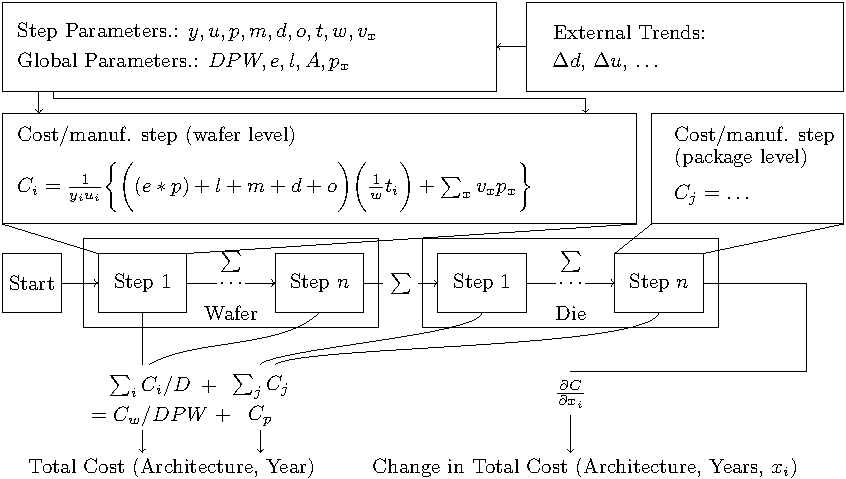
\includegraphics[width=0.95\textwidth]{./figures/costmodel.pdf}
    \caption{\textbf{Cost model structure.} The diagram shows inputs to each step and computational steps leading to the cost model outputs. For the description of cost variables, see definitions for \cref{eqn:cost_wafer}.}
    \label{fig:costmodel-schematic}
\end{figure}

\begin{figure}[h!]
    \centering
    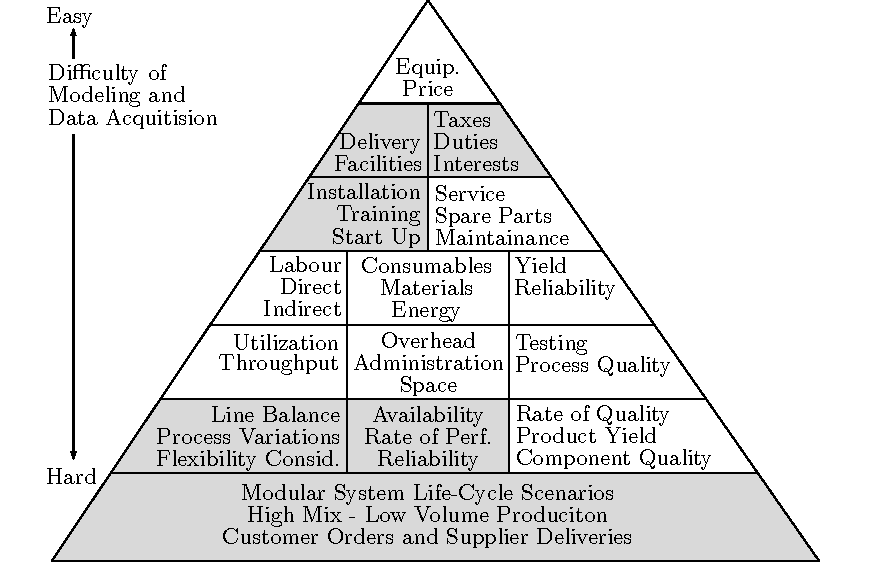
\includegraphics[width=0.85\textwidth]{./figures/SEMI_pyramid.pdf}
    \caption{\textbf{\textit{SEMI Standard 35} pyramid showing variables that enter into the computation of manufacturing cost in our model.} Variables not captured by our model are greyed out. The pyramid has been adapted from \cite{standardE35} and \cite{helin200618th}.}
    \label{fig:semi_pyramid}
    \vspace{-20mm}
\end{figure}

\clearpage

As illustrated in \cref{fig:semi_pyramid}, our model is comprehensive in its coverage of market, economic, manufacturing step and global manufacturing parameters. However, the model has limitations which must be considered when interpreting the results:

\textbf{Availability of Equipment Performance Data for all Chip Architectures}

The data for the inputs used in the model were obtained through a combination of scientific literature, conference proceedings, industry reports, industry periodicals, manufacturing equipment datasheets and experts interviews. The model was therefore set up to consider four light-emitting diode chip architectures: A classical light-emitting diode chip architecture with lateral current spreading, two different high-power thin-film flip-chip architectures and a chip-scale package thin-film flip chip architecture, all shown in \cref{sec:manufacturing_steps}.

Unfortunately, despite the multitude of data sources, important performance parameters of  manufacturing equipment relevant to the latest generation of chips, such as those shown in \cref{fig:manuf_vtf_2012-1}-\cref{fig:manuf_csp_2020-2}, were unavailable due to their highly proprietary nature. Since full coverage of manufacturing equipment performance parameters could therefore not be assured for all chip architectures, costs were computed only for the aforementioned classical chip architecture.

\textbf{Lack of Data for Calibration}

Due to limitations in data availability, the cost model is set up to capture the cost structure of a hypothetical factory employing the most up-to-date equipment in every model year. It operates at a fixed-cost basis (labor cost, electricity cost, cleanroom cost, etc.). However, this does not correspond to any \textit{real, physical} location. The majority of production capacity is presently located in Asia. There, the share of domestically produced manufacturing equipment has increased from 10\% in 2008 to 65\% in 2015 \cite{tseng2015fab}. Recent investments into factories for high-power light-emitting diodes include Osram's Kulim plant in Malaysia \cite{osram2020kulim} and Lumileds' Penang plants in Malaysia \cite{lumileds2020penang}. In the production of low-power light-emitting diodes, the world's largest producer of LED packages by volume, MLS Co. operates plants in mainland China \cite{mls2020dev}. This means that it is difficult to validate model outputs directly with the help of industry data, which (even for American and European companies) is provided only for Asia-based manufacturing lines. 

Generally, we found that our model provides the best-case scenario for LED manufacturing, where the most performant (highest throughput, highest yield) equipment is used in each year. Interviews revealed that this is rarely the case in practice. One reason for this is additional economic pressure on western manufacturers following the introduction of significant Chinese subsidies as part of the country's Twelfth Five-Year Plan \cite{sanderson2014light}. While in reality, older equipment with lower performance might be used, we model the use of the best available equipment for each year considered.

Because the purpose of our model is to show the impact of changes in the design and manufacturing process of devices, rather than the geographic location and associated economic circumstances, we believe this to be a minor drawback. For fixed cost parameters, we therefore assumed a US-based manufacturing environment. We do compare cost model data to a selection of industry data in \cref{sec:cost_model_calibration} and provide an interpretation of the differing cost structure.

Unfortunately, benchmarking the total cost computed with our model against industry data is not possible. While the US Department of Energy has managed to convince companies to share their cost structure (shown in Supplementary Figure 16), they never share \textit{absolute} cost. The closest industry publication ever comes to disclosing absolute cost data is in their reporting data on \$/klm at the chip-level. Our model (like most other manufacturing cost models we reviewed) computes only the total manufacturing cost, since a combined computation of cost and performance would require a highly complex treatment not only of the cost associated with equipment performance, but also of the associated changes in the bulk semiconductor, phosphor, packaging, etc. To the best of our knowledge, this has not been attempted, at least in a publicly available fashion, for solid-state lighting devices.

\clearpage
\subsection{Yielded Cost}
\label{sec:cost_computation}

The manufacturing process of semiconductor devices can be categorized by the level at which manufacturing process steps are implemented, i.e., either at the wafer level or at the individual chip/package level. The total manufacturing cost per die is thus the sum of the total costs of all wafer processing steps and all die packaging steps.
%
\begin{equation}
\label{eqn:cost_sum}
    C \bigg[ \frac{ \text{USD}(2020) }{ \text{die} } \bigg] = P_S + C_w + C_p
\end{equation}
%
where
%
\begin{align*}
    P_S &\dots \text{sapphire substrate price per die} \\
    C_w &\dots \text{wafer processing cost per die} \\
    C_p &\dots \text{die processing cost}
\end{align*}
%
The total wafer processing cost and total die packaging costs are in turn the sum of all associated process steps.
%
\begin{equation}
        C_w = \sum_i C_i
\end{equation}
%
\begin{equation}
	C_p = \sum_j C_j
\end{equation}
%
The cost of a single process step $C_i$ can now be written as
%
\begin{equation}
\label{eqn:cost_wafer}
    C_i \bigg[ \frac{ \text{USD}(2020) }{ \text{die} } \bigg] =\frac{1}{DPW}  \frac{1}{y_i}   \bigg\{ \bigg((c_e*p) + c_l + c_m + c_d + c_o \bigg)_i \bigg( \frac{t_i}{w_i u_i} \bigg) + \sum_{x} v_x c_x \bigg\}
\end{equation}
%
where the index $i$ runs over all wafer processing steps, the index $j$ runs over all die processing steps and the index $x$ run over all materials.
%
\begin{align*}
        DPW &\dots \text{number of functional (i.e., successfully tested) die per wafer}\\
        y &\dots \text{process step yield} \\
        u &\dots \text{equipment utilization (relative to theoretical equipment capacity)} \\
        p &\dots \text{power consumption} \\
        c_e &\dots \text{hourly electricity cost} \\
        c_m &\dots \text{hourly maintenance cost} \\
        c_d &\dots \text{hourly depreciation cost}\\
        c_l &\dots \text{hourly labour cost} \\
        c_o &\dots \text{hourly overhead cost} \\
        t_i &\dots \text{time per run} \\
        w &\dots \text{wafers per run} \\
        v_x &\dots \text{volume of material $x$ per wafer} \\
        c_x &\dots \text{cost of material $x$ per volume}\\
\end{align*}
%
The number of die per wafer $D$ depends on the total usable wafer area $A_{\text{usable}}$. The usable area depends on the total area of the wafer $A_{\text{wafer}}$ , the cutting street width area between the chips $A_{\text{cut}}$  and the exclusion zone at the rim of the wafer $A_{\text{exclusion}}$ .
%
\begin{equation}
	A_{\text{usable}}=A_{\text{wafer}}-A_{\text{cut}}-A_{\text{exclusion}}
\end{equation}
%
Determining the usable wafer area as a function of these three parameters requires a numerical solution. However, following discussions in the literature \cite{de2005investigation}, we approximate the number of functional die per wafer\footnote{often \textit{"good die per wafer"} in the literature} as
%
\begin{equation}
\label{eqn:dpw}
	DPW = \frac{\pi}{4}  \bigg ( \frac{d-2e}{\sqrt{a}+s/2} \bigg ) ^2 - \frac{\pi}{\sqrt{2}}\frac{d-2e}{(\sqrt{a}+s/2)^2}
\end{equation}
%
where
%
\begin{align*}
    d &\dots \text{wafer diameter} \\
    e &\dots \text{wafer edge exclusion zone width} \\
    a &\dots \text{die area} \\
    s &\dots \text{cutting street width} \\
\end{align*}

\cref{fig:dpw} shows the results of DPW calculations using \cref{eqn:dpw} for different wafer diameters $d$ that were most commonly used in LED manufacturing in 2003 (50mm), 2010 (100mm) and 2020 (200mm). We can see that DPW dramatically increases over time.

\begin{figure}[h!]
    \centering
    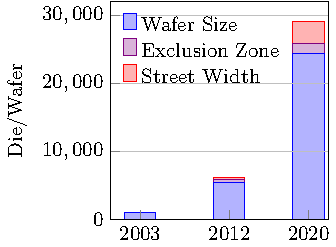
\includegraphics[width=5.5cm]{./figures/die-per-wafer.pdf}
    \caption{\textbf{Number of die per wafer for the dominant wafer diameters used in different years.} $d(2003)=50$mm$\rightarrow851$ DPW, $d(2010)=100$mm$\rightarrow5370$ DPW, $d(2020)=200$mm$\rightarrow26,838$ DPW. Source: own estimates, based on \cref{eqn:dpw} and the dominant wafer size of the considered year, informed by expert interviews. For detailed statistics on changes in wafer size, compare also \cref{fig:wafers}.}
    \label{fig:dpw}
\end{figure}

\cref{eqn:cost_wafer_full} then gives us for the cost of a manufacturing step $C_i$ in the wafer processing category
%
\begin{equation}
\label{eqn:cost_wafer_full}
\begin{split}
    C_i \bigg[ \frac{ \text{USD}(2020) }{ \text{die} } \bigg] &= \bigg (  \frac{\pi}{4}  \bigg ( \frac{d-2e}{\sqrt{a}+s/2} \bigg ) ^2 - \frac{\pi}{\sqrt{2}}\frac{d-2e}{(\sqrt{a}+s/2)^2} \bigg )^{-1} \times \\
    &  \frac{1}{y_i}  \bigg\{ \bigg((c_e*p) + c_l + c_m + c_d + c_o \bigg)_i \bigg( \frac{t_i}{w_i u_i} \bigg) + \sum_{x} v_x c_x \bigg\}
\end{split}
\end{equation}
%
and the cost of a manufacturing step $C_j$ in the packaging category
%
\begin{equation}
\label{eqn:cost_die}
    C_j \bigg[ \frac{ \text{USD}(2020) }{ \text{die} } \bigg] = \frac{1}{y_j}  \bigg\{ \bigg((c_e*p) + c_l + c_m + c_d + c_o \bigg)_i  \frac{c_j}{u_j} + \sum_{x} a v_x c_x \bigg\}
\end{equation}
where $c_j$ is $\text{throughput}^{-1}$. The total cost is thus
%
\begin{equation}
\label{eqn:cost_total}
\begin{split}
    C= P_s &+ \sum_i \bigg \{ \frac{1}{DPW} \frac{1}{y_i} \bigg[ \frac{t_i}{w_i u_i} \bigg((e*p) + l + m + d +o \bigg)_i  + \sum_{x} v_x p_x \bigg] \bigg \} + \\
    & + \sum_j \bigg \{ \frac{1}{y_j} \bigg[ \frac{c_j}{u_j}  \bigg((e*p) + l + m + d + o \bigg)_i + \sum_{x} a v_x p_x \bigg ] \bigg\}
\end{split}
\end{equation}

\textbf{Computation of Yielded Cost}

Devices may be damaged or otherwise rendered unusable during the manufacturing process. The ratio between the number of good devices per step and the number of handled devices per step is known as the yield. Optimizing this yield is critical for reducing manufacturing cost \cite{Kumar2006}. This is because cumulative yield quickly drops as the yield from manufacturing steps with below 100\% yield compounds. We must thus consider not only the manufacturing cost per process step, but also the cost including the yield \cite{becker2001use}\cite{becker2001using}. While there are different mathematical approaches to including yield, we follow the definition in \cite{becker2001use}. We write for the yielded cost $C_{Y_i}$ of a step $i$ with associated cost (before considering yield) $C_1$ and yield $Y_1$, starting from steps $1,2,\dots,i$:
%
\begin{equation}
\label{eqn:C_2}
    C_{Y_1} = \frac{C_1}{Y_1}
\end{equation}
\begin{equation}
    C_{Y_2} = \frac{C_1 + C_2}{Y_1 Y_2} - C_{Y_1} = \frac{C_1 + C_2}{Y_1 Y_2} - \frac{C_1}{Y_1} = \frac{1}{Y_1 Y_2} \bigg ( C_1 (1-Y_2) +C_2 \bigg)
\end{equation}
\begin{equation}
    C_{Y_i} = \frac{ \sum_{x \leq i} C_x }{ \prod_{x \leq i} Y_x } - \frac{ \sum_{x<i} C_x }{ \prod_{x<i} Y_x }
\end{equation}
%
If a step is applied more than once, we can conveniently rewrite this in a form suited to computation within the \textit{Excel} worksheet. Assuming step $2$ is used twice, we get for the yielded cost of this step an equation of the form
%
\begin{equation}
\label{eqn:C_2^2}
    C_{Y_2}^{(2 \times)} = \bigg( \frac{C_1 + C_2}{Y_1 Y_2} - \frac{C_1}{Y_1} \bigg) + \bigg( \frac{C_1 + 2 C_2}{Y_1 Y_2^2} - \frac{C_1 + C_2}{Y_1 Y_2}     \bigg)
\end{equation}
%
\begin{equation}
    = \frac{1}{Y_1 Y_2^2} \bigg( C_1 (1-Y_2^2) +2C_2 \bigg)
\end{equation}
%
which can be compared to  \cref{eqn:C_2} to find a more general form:
%
\begin{equation}
    C_{Y_2}^{(n \times)} = \frac{1}{Y_1 Y_2^n} \bigg( C_1 (1-Y_2^n)+nC_2\bigg)
\end{equation}
%
It can be shown by induction that the general form of a term for a step $i>1$ repeated $n$ times can be expressed as:
%
\begin{equation}
\label{eqn:yielded_cost}
    C_{Y_{i>1}}^{(n \times)} = \frac{1}{Y_i^{n-1} \prod_{x \leq i} Y_x} \bigg( nC_i + \sum_{x < i} C_x (1-Y_i^n) \bigg)
\end{equation}
%
This cumulative approach to yielded cost is different from the approach taken in the original \textit{LEDCOM} model \cite{ledcomv2}. It uses what in the literature is described as an \textit{"itemized approach"} to yielded cost \cite{becker2001use}. In this approach, the yielded cost of a single process step $f$ is described as
%
\begin{equation}
    f_\text{single} = \frac{k+s}{y}
\end{equation}
%
where
%
\begin{align*}
    k &\dots \text{material cost of previous step} \\
    s &\dots \text{step cost}
\end{align*}
%
For process steps that are performed more than once, a series expression is used
%
\begin{equation}
    f_{\times 2} =  \frac{\frac{k+s}{y}+s}{y}
\end{equation}
\begin{equation}
\label{eqn:series}
    f_{\times n} = \frac{k + s(1+y+y^2+ \dots + y^{n-1})}{y^n}
\end{equation}
%
This itemized approach serves as a convenient approximation, but its cumulative contributions do not equal the total yielded cost of the entire manufacturing process
%
\begin{equation}
    f_\text{total} = \frac{\sum_i^n s_k}{\prod_i^n y_i} \neq \sum_i^n f_i
\end{equation}
%
where $n$ is the total number of steps. This is due to the approximation introduced in \cref{eqn:series}.

\textbf{Input Data on Sapphire Wafers}

Sapphire wafers form the substrate on which all other layers of the light-emitting diode are grown. Being transparent to radiation in the visible spectrum, it is not removed after growth in the Classical architecture or the Thin-Film Flip-Chip architecture. In the Vertical Thin-Film architecture, it is removed by means of a laser-lift-off process. Wafers can be either unpatterned or patterned, where the latter has become commonplace by 2020 due to the beneficial properties that microstructures on the surface have on layer growth \cite{wuu2009defect} and light-extraction efficiency \cite{lee2006enhancing}. The price of sapphire substrates has decreased significantly since the year 2000, as shown in the top panel of \cref{fig:wafers}. This can be attributed not only to their role in the solid state lighting industry, but more importantly to increased supply in response to increased demand from electronics manufacturing \cite{yole2015sapphire}, where sapphire glass is used to protect screens and sensor interfaces from scratches \cite{khattak2016world}.

Wafer sizes used in manufacturing have also increased over the years due to favourable economics of large wafer processing (see bottom panel in \cref{fig:wafers}). The market has been dominated by U.S.-based \textit{Rubicon Technology} and Russian-based \textit{Monocrystal}. We use the market average for the sapphire wafer price in different years as a direct input into the cost model, and the dominant wafer diameter (see bottom panel in \cref{fig:wafers}) in different years as an input to calculate DPW in \cref{eqn:dpw}.

\begin{figure}[h!]
    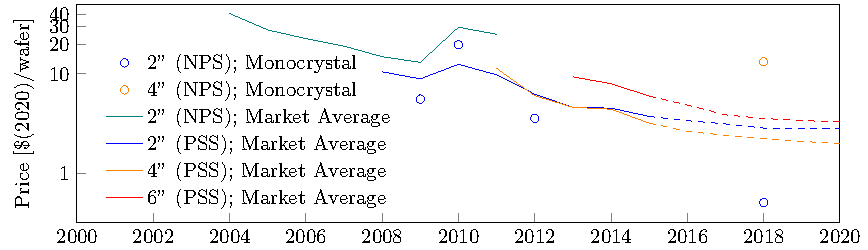
\includegraphics[width=15cm]{./figures/sapphire_prices.pdf}
    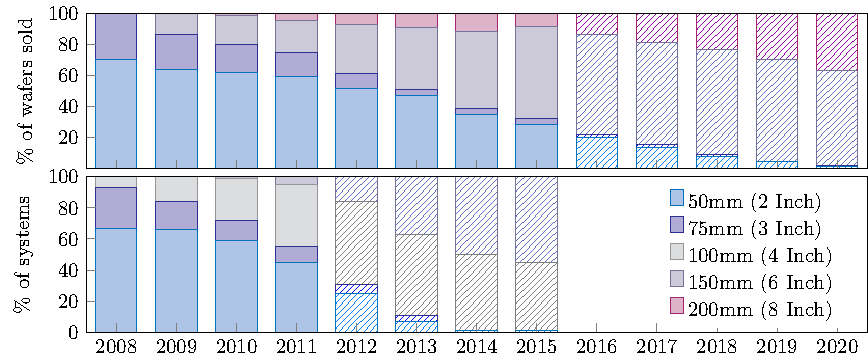
\includegraphics[width=14.5cm]{./figures/wafer_size.pdf}
	\caption{\textbf{Historical trends in sapphire wafer size and price.} Top panel: Historical data for sapphire substrate prices of different surface properties and diameters, 2004-2020. Shown is data for non-patterned (polished) surface (NPS) and patterned surface substrates (PSS). Monocrystal denotes the Russian manufacturer of the same name. Dashed lines are projections made in 2015. Sources: \cite{monocrystal2020private}\cite{yole2011sapphire}\cite{yole2015sapphire}. Bottom panel: Prevalence of sapphire wafer size used in LED manufacturing in 2008-2020. Hatched bars are projections. Sources: \cite{veeco2013}\cite{Scholand2012}\cite{yole2015sapphire}}
	\label{fig:wafers}
\end{figure}

\subsection{Contribution of Variables}
\label{sec:contribution_variables}

To quantify the drivers of changes in manufacturing cost or device performance among many contributing factors, one would need to identify the magnitude of contribution to these changes made by single variables in equations \cref{eqn:cost_wafer} and \cref{eqn:cost_die}. Mathematically, given a function $F$ which describes the manufacturing cost or performance function of a device at time $t$,
%
\begin{equation}
F=ab+cd
\end{equation}
%
and input variables $a,b,c,d$, we are looking for the contribution $\Delta F_{a}$ made by a single variable $a$ to the total change in the function value $\Delta F$ between points $t_0,t_1$ such, that
%
\begin{equation}
\Delta F = F(t_1)-F(t_0) = \sum_{i=a, \dots, d} \Delta F_i
\end{equation}
%
Index decomposition analysis has been developed to solve this problem \cite{Boyd1987}. A short derivation, based on \cite{kavlak2018evaluating} is provided below.

The infinitesimal contribution to the total function value by the infinitesimal change in an input variable is defined through the total differential of the function as
%
\begin{equation}
\text{d}F(x_1 (t), x_2(t), \dots) = \sum_i \frac{\partial F }{\partial x_i}     \frac{\text{d}x_i}{\text{d}t} = \sum_i \frac{\partial F }{\partial x_i}  \Delta x_i
\end{equation}
%
where $x_i$ is an input variable. The contribution of the change $\Delta x_1$ in variable $x_1$ to the total function value $F$ over the period $t_0 < t < t_1 $ is then
%
\begin{equation}
\Delta F_{x_1} = \int_{t=t_1}^{t_2} \frac{\partial F }{\partial x_1} \frac{\text{d}x_1}{\text{d}t} \text{d}t
\label{eqn:integral_1}
\end{equation}
%
However, data on the input variables in our study is often not available in continuous time. Disaggregating the contribution of single variables to the change in the cost or performance is thus not straightforward in our model. This problem does not arise in cost models which compute cost changes directly, such as \cite{nemet2012solar} \cite{goodrich2013assessing}. In our work, we propose to address this problem by following an approach developed by Kavlak et al. \cite{kavlak2018evaluating}. For the detailed derivation, we refer to this publication.

In this approach, the function $F$ as a function of a vector of input model variables $\vec{r}=(r_1,r_2,\dots)$ is defined as
%
\begin{equation}
    F(\vec{r}) = F(r_1,r_2, \dots) = \sum_i F_i
\end{equation}
where
\begin{equation}
    F_i(\vec{r}) = F_i^0 \prod_w g_{iw}(r_w)
\end{equation}
%
which can be written as a constant part $F$ and a part describing the dependence of the $i$-th cost component on the $w$-th variable.
%
Using logarithmic differentiation, the integral from  \cref{eqn:integral_1} can be rewritten as
\begin{equation}
    \Delta F_x = \int_{t=t_0}^{t_1} F(t) \frac{ \partial \ln F }{ \partial x } \frac{ \text{d} x }{ \text{d} t} \text{d} t
\end{equation}
%
where for $F(t)$ a constant $F(t) \approx \tilde{F} $ can be chosen such that $\Delta F_{x_i} = \Delta F$. In practice, this constant value can be approximated through the geometric and arithmetic means $\tilde{F} \approx \frac{2}{3} F_i^\text{geo} + \frac{1}{3} \overline{F_i}$ \cite{kavlak2018evaluating}. The contribution of a single cost model variable $r_z$ can then be written as
%
\begin{equation}
    \Delta F_z (t_1,t_2) \approx \sum_i \tilde{F_i} \ln \frac{g_{iz}(t_2)}{g_{iz}(t_1)}
\end{equation}
%
We use this approach to estimate the effect of individual innovations and spillovers on LED device performance, as discussed in relation to Figure 5 in the main article. Due to time constraints, we leave the quantification of the impact of different drivers of cost reductions with this methodological approach for our future work.

\clearpage

\section{Supplementary Discussion}

\subsection{Cost Model Sensitivity Analysis}

\begin{figure}[ht!]
	\centering
    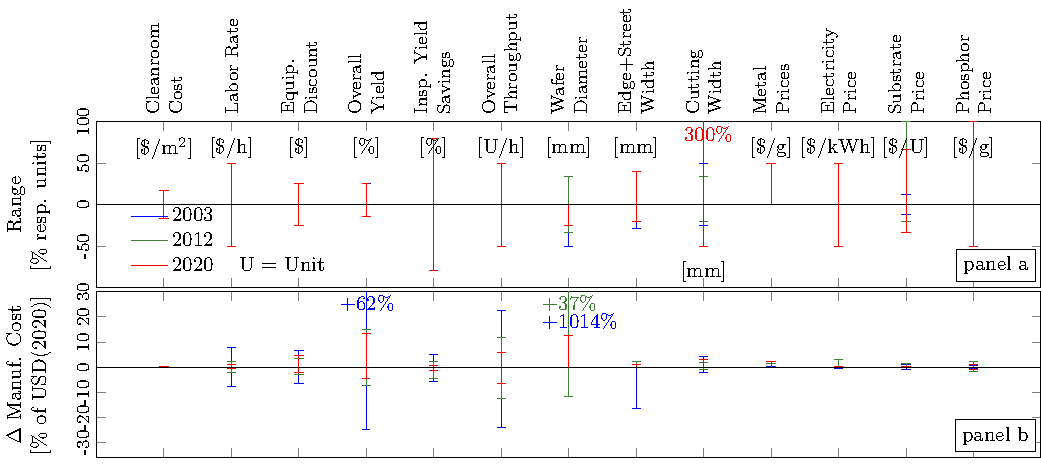
\includegraphics[width=\textwidth]{./figures/costmodel_sensitivity.pdf}
	\caption{\textbf{Sensitivity analysis for selected cost model parameters.} Panel a represents the tested range of variation of parameters indicated on horizontal axis along with their respective measurement units, as represented in Supplementary Table 3. Panel b shows the resulting range of variation in the manufacturing cost. Ranges are represented for three years considered in the cost model, where corresponding data is available, by whiskers of the following colour: 2003 – blue, 2012 – green, 2020 – red. Note the overall trend of decreasing sensitivity to cost model parameters as the number of die per wafer increases over time. Abbreviations: resp. - respective; Yield Sav. from Insp. - yield savings from inspection.}
	\label{fig:sensitivity}
\end{figure}

A sensitivity analysis of the cost model has been performed using parameter variations listed in table \cref{tab:sensitivity}. The amount of parameter variation was chosen to encompass the identified range of parameter values in different manufacturing setups for each considered year. As an example, the lower range in the variation for the price of metals used in the model (+50\%,-0\%) was chosen based on the prices quotes from the United State Geological Survey price database \cite{usgeoprices}. Industry metals are not sold below the price of the raw material and often the markup is small compared to the price of the material. The upper range was chosen because a survey of industrial metal suppliers for semiconductor manufacturing showed that the largest markup was below 50\%. The results of the analysis are shown in  \cref{fig:sensitivity}. The cost model is generally more sensitive to the variation in parameters at smaller wafer diameters. The most sensitive parameters are global parameters, such as yield or average equipment throughput.

\begin{table}[]
\centering
\small
    \caption{\textbf{List of cost model parameters considered in sensitivity analysis.}}
    \begin{NiceTabularX}{1.1\textwidth}{ |X|X|l|l|l|l|l|l|X|}
        \hline
            \textit{Parameter} & \textit{Unit} & \textit{2003} & $\pm [\%]$ & \textit{2012} & $\pm [\%]$ & \textit{2020} & $\pm [\%]$ & Source \\
        \hline
            Cleanroom Cost & \text{USD}/m$^2$ & 3000 & +16,-16 & 3000 & +16,-16 & 3000 & +16,-16 & \cite{mddi1997cleanroom}\cite{ledcomv2} \newline \cite{bakshi2009euv}\cite{gajera2006process} \\
        \hline
            Labor Rate & \$/h & 30 & +50,-50 & 30 & +50,-50 & 30 & +50,-50 & I \\
        \hline
            Equip. Discount & \% of \text{USD} & 0\% & +25,-25 & 0\% & +25,-25 & 0\% & +25,-25 & I \newline \cite{Appleyard_2001} \\
        \hline
            Overall Yield & \% & 31\% & +25,-25 & 57\% & +25,-15 & 74\% & +25,-25 & I, \cite{lumi2012yield}\cite{ledsmag2012} \newline \cite{systemplus2015reverse}\cite{ledcomv2} \\
        \hline
            Inspec. Yield Savings & \%/inspec. & 0.5\% & +80,-80 & 0.5\% & +80,-80 & 0.5\% & +80,-80 & \cite{mckinseyyield} \\
        \hline
            Overall Throughput & UPH or h$^{-1}$ & varies & +50,-50 & varies & +50,-50 & varies & +50,-50 & Equipment Datasheets \\
        \hline
            Wafer Diameter & mm & 100 & +0,-50 & 150 & +33.3,-33.3 & 200 & +0,-25 & I and \cref{fig:wafers} \\
        \hline
            Edge+Street Width & mm & 7 & +0,-50 & 5 & +40,-0 & 5 & +40,-20 & \cite{ledsmagexclusion}\cite{rubiconexclusion} \newline \cite{xiamenexclusion}\cite{american2007annual} \\
        \hline
            Cutting Width & $\mu$m & 100 & +50,-25 & 75 & +33.3,-20 & 20 & +300,-50 & \cite{masaki2000division}\cite{ils2005width} \newline \cite{photonics2010width}\cite{discowidth} \\
        \hline
            Metal Prices & \text{USD}/kg & varies & +50,-0 & varies & +50,-0 & varies & +50,-0 & Datasheets \\
        \hline
            Electricity Price & \text{USD}/kWh & 0.07 & +50,-50 & 0.08 & +50,-50 & 0.06 & +50,-50 & \cite{eia2000electric}\cite{eia2019electric} \\
        \hline
            Saph. Subst. Price & \text{USD} & 40 & +12.5,-12.5 & 10 & +100,-20 & 3 & +66.6,-33.3 & \cref{fig:wafers} \\
        \hline
            Phosphor Prices & \text{USD}/g & varies & +50,-50 & varies & +0,-0 & varies & +0,-0 & I, \cite{yole_phosphor_2012}\cite{yole2017phosphor} \\
        \hline
        \end{NiceTabularX}
    \vspace{2mm}
    \caption*{The results of the sensitivity analysis for the parameters in this table are presented in \cref{fig:sensitivity}. Note: Baseline values are provided only for \textit{global} model parameters in the columns \textit{2003, 2012, 2020}. For \textit{non-global} model parameters (those which vary by equipment) only the variation, in percent of the individual baseline values is provided. The corresponding units for the values in columns \textit{2003}-\textit{2020} are indicated in the column \textit{Units}. The variation employed during the sensitivity analysis is provided in the columns $\pm [\%]$. Abbreviations: UPH - units per hour; Equip. Discount - equipment discount (sales rebate for large purchases); Inspec. Yield Savings - yield savings from inspection (early detection and alleviation of issues in the manufacturing workflow); Saph. Subst. - Sapphire Substrate. ’I’ in the Source column indicates expert interviews as the source of information.}
    \label{tab:sensitivity}
\end{table}

\clearpage
\subsection{Cost Data Comparison with Industry Projections}
\label{sec:cost_model_calibration}

In order to validate the outputs of the cost model regarding the evolution of the cost structure of low-to-mid-power classic chip GaN phosphor-converted white LED, we conducted a comparison with previously reported U.S. DOE calculations and projections based on the \textit{LEDCOM} model and industry data provided as part of industry round table discussions:

\begin{figure}[h]
	\centering
    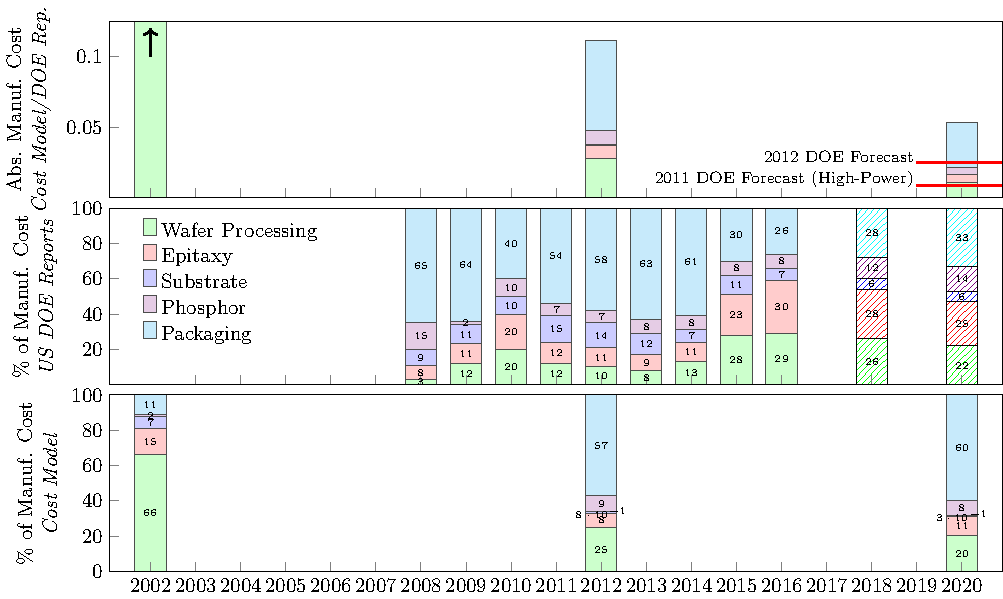
\includegraphics[width=\textwidth]{./figures/costmodel_calibration.pdf}
	\caption{\textbf{Cost structure comparison between our cost model, industry data and DOE projections.} Top panel: Absolute manufacturing cost, with two U.S. DOE projection for context. Center panel: manufacturing cost calculations (2008-2016) and projections (2018, 2020) previously published by the U.S. DOE based on industry data and LEDCOM model. Bottom panel: manufacturing cost structure produced by our cost model for 2002, 2012 and 2020. Hatched bars are DOE projections. Sources for top/center panel: \cite{doe2010solid}\cite{doe2011solid}\cite{doe2012solid}\cite{doe2013solid}\cite{doe2014solid}\cite{doe2015solid}\cite{doe2016solid}. Sources for bottom panel: own elaboration based on the cost model described in \cref{sec:costmodel_structure}.}
	\label{fig:costmodel_calibration}
\end{figure}

\textbf{}
We note some differences between the results of our model and the cost structure reported or projected by the DOE. For instance, the share of the epitaxy step is consistently larger in the DOE data. This can in part be explained by our model assuming the use of state-of-the-art equipment, while industry might not run low-power and mid-power chip production on these more expensive reactors. In addition, the manufacturing lines of the majority of manufacturers are located in Asia. We also note that the share of the sapphire substrate price in the DOE data is much larger than in our model, which can in part be explained by the overestimation of the actual price of sapphire wafers in earlier projections made for 2015-2020. Finally, the relative importance of the packaging part of the manufacturing process is very similar in our model and in the DOE results in 2012. However, in the DOE projections it significantly decreases by 2020, while in our model it retains and even increases its share of the total cost. This trend has been independently confirmed by researchers and industry reports on wafer-level packaging \cite{Lee2011WPL,Xie2013,ledsmag2017WLP}, showing better performance of our cost model compared to earlier DOE model projections.

\clearpage
\addcontentsline{toc}{section}{Supplementary References}
\printbibliography[title=Supplementary References]

\end{document}